%\VignetteIndexEntry{REST Guide} \\
%\VignetteEngine{knitr::knitr}

\documentclass[a4paper]{article}\usepackage[]{graphicx}\usepackage[]{color}
%% maxwidth is the original width if it is less than linewidth
%% otherwise use linewidth (to make sure the graphics do not exceed the margin)
\makeatletter
\def\maxwidth{ %
  \ifdim\Gin@nat@width>\linewidth
    \linewidth
  \else
    \Gin@nat@width
  \fi
}
\makeatother

\definecolor{fgcolor}{rgb}{0.345, 0.345, 0.345}
\newcommand{\hlnum}[1]{\textcolor[rgb]{0.686,0.059,0.569}{#1}}%
\newcommand{\hlstr}[1]{\textcolor[rgb]{0.192,0.494,0.8}{#1}}%
\newcommand{\hlcom}[1]{\textcolor[rgb]{0.678,0.584,0.686}{\textit{#1}}}%
\newcommand{\hlopt}[1]{\textcolor[rgb]{0,0,0}{#1}}%
\newcommand{\hlstd}[1]{\textcolor[rgb]{0.345,0.345,0.345}{#1}}%
\newcommand{\hlkwa}[1]{\textcolor[rgb]{0.161,0.373,0.58}{\textbf{#1}}}%
\newcommand{\hlkwb}[1]{\textcolor[rgb]{0.69,0.353,0.396}{#1}}%
\newcommand{\hlkwc}[1]{\textcolor[rgb]{0.333,0.667,0.333}{#1}}%
\newcommand{\hlkwd}[1]{\textcolor[rgb]{0.737,0.353,0.396}{\textbf{#1}}}%

\usepackage{framed}
\makeatletter
\newenvironment{kframe}{%
 \def\at@end@of@kframe{}%
 \ifinner\ifhmode%
  \def\at@end@of@kframe{\end{minipage}}%
  \begin{minipage}{\columnwidth}%
 \fi\fi%
 \def\FrameCommand##1{\hskip\@totalleftmargin \hskip-\fboxsep
 \colorbox{shadecolor}{##1}\hskip-\fboxsep
     % There is no \\@totalrightmargin, so:
     \hskip-\linewidth \hskip-\@totalleftmargin \hskip\columnwidth}%
 \MakeFramed {\advance\hsize-\width
   \@totalleftmargin\z@ \linewidth\hsize
   \@setminipage}}%
 {\par\unskip\endMakeFramed%
 \at@end@of@kframe}
\makeatother

\definecolor{shadecolor}{rgb}{.97, .97, .97}
\definecolor{messagecolor}{rgb}{0, 0, 0}
\definecolor{warningcolor}{rgb}{1, 0, 1}
\definecolor{errorcolor}{rgb}{1, 0, 0}
\newenvironment{knitrout}{}{} % an empty environment to be redefined in TeX

\usepackage{alltt}
\usepackage[margin=2cm]{geometry}
%\usepackage{Sweave}
\usepackage{graphicx}
\usepackage{amsmath}
\usepackage{amssymb}
\usepackage{color}
\usepackage{setspace}
\usepackage{multirow}
\usepackage{float}
\usepackage[english]{babel}
\usepackage{natbib}

\usepackage{hyperref}
\hypersetup{
	colorlinks, 
	citecolor=black,
	filecolor=black,
	linkcolor=black,
	urlcolor=black
}


\title{RcmdrPlugin Easy Script Templates 1.0.0}
\author{Ewoud De Troyer}
\date{}
\IfFileExists{upquote.sty}{\usepackage{upquote}}{}
\begin{document}

\maketitle
\tableofcontents
\newpage
\section{Introduction}
R is a great platform for statisticians to do their analyses and data
manipulation. Thanks to the existence of R packages, new code can be easily
distributed and executed by other statisticians.\\
However for other scientists, the barrier to understand the coding language of
R, can sometimes be too difficult to breach. This is a shame since it means that
all of the implemented methodology in R, is inaccessible for them. One way to
bridge this gap is through the use of {\it Graphical User Interfaces} (GUI). While the R-code is
still responsible for the analyses in the background, the user does not need to
worry about it since the methods can be accessed through simple point and click.
\\ \\
However making a GUI can take up quite some time. Learning the syntax of
creating windows, creating the actual code, etc. Sometimes there is simply no
time left to invest in this exercise. This is where the \texttt{REST} package (or
\texttt{{\bf R}cmdrPlugin {\bf E}asy {\bf S}cript {\bf T}emplates}) comes into
play. \texttt{REST} contains an easy script template to create new dialogs in
the form of a plug-in for R Commander (\texttt{Rcmdr}). These scripts do not
require any knowledge about \texttt{tcltk} or \texttt{Rcmdr} and are very
straightforward to use. They will allow developers to translate the R-code from
their packages into a GUI without too much difficulty.\\
This means that the \texttt{REST} is not meant to be used independently. It
should be imported or depended upon in your own GUI package.
\\ \\
{\it R Commander} was chosen as the starting platform for the GUI's since it
will also show the R code (from the package the GUI is based on) going on in the
background. For example, if the user would click on a plot button, the original
code `\texttt{plot(...)}' would appear in the script window. Users can simply
decide to ignore this or, even better, use it to start learning the syntax of R
while using GUI's.
\\ \\
It should be mentioned that the scripts used in this package are a
generalisation of the templates scripts which were used in the
\texttt{RcmdrPlugin.BiclustGUI} package.

\section{R Commander}

R Commander, \verb|Rcmdr|\citep{Fox2005}, is a GUI developed by John Fox from
McMaster University, Canada. Originally it was conceived as a basic-statistics graphical
user interface for R, but its capabilities have been extended substantially
since. The \verb|Rcmdr| package is based on the \verb|tcltk| package
\citep{Dalgaard2001} which provides an R interface to the {\it Tcl/Tk} GUI builder. 
Since \verb|tcltk| is available on all the operating systems on which R is
commonly run, the R Commander GUI will also run on all of these platforms.\\ \\
The GUI is also very easy to start to use for beginners who do not have any
or little experience with R. It will protect beginners from errors as the dialog
boxes only have limited options related to the current context. Further, since
the users are exposed to the actual R commands through a script and output
window, besides analyzing and managing the data in R easily, they can also
learn how do it in R without a GUI.
Another advantage is that the script will be generated on the fly as the user
applies the desired statistics through the point-and-click GUI. This means it can be easily
saved at the end of a session which enables the user afterwards to recreate the
results by running the R script without going through all the dialogs again.
Advanced users can even adapt the created script to do some more detailed
analysis. These are the main advantages \verb|Rcmdr| has over other available
RGUI packages.\\ \\
Starting with version 1.3-0, \verb|Rcmdr| also provides the possibility of {\it
plug-in} packages which can augment the R Commander menus. These packages are
developed, maintained, distributed and installed indepently of \verb|Rcmdr| and
can provide a wide variety of new dialog boxes and statistical functionality.
More information on developing such a plug-in can be found in \citet{Fox2007}.\\

\begin{figure}[H]
\centering
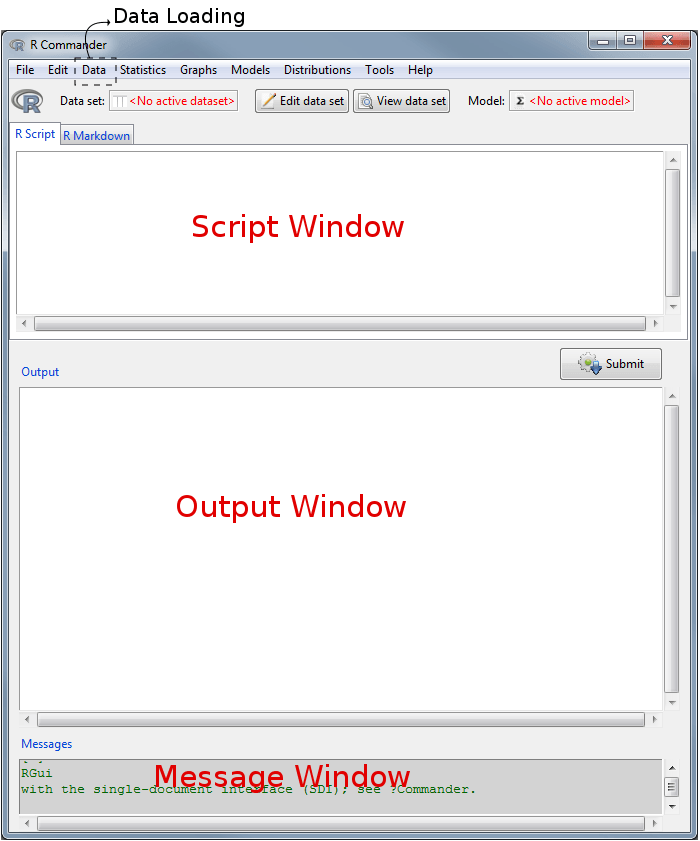
\includegraphics[width=10cm]{figures/rcmdrwindow.png}
\caption{{\it Default R Commander}\label{rcmdrwindow}}
\end{figure}


\section{Other GUI Creation Packages}
There exist several packages in R to help users create GUI's. Some examples are
\verb|Rgtk2| \citep{Lawrence2014} and \verb|gWidgets| \citep{Verzani2014}.
Especially the latter already operates at a fairly high level to help users
create quick and interactive GUI's without too much fuss. The \verb|REST|
package differs in that it works on an even higher level by using a
``fill-out'' script. This reduces the learning curve even more. The
price to pay however is that it is less flexible than than a package like
\verb|gWidgets|.\\
Another difference lies in the fact that \verb|REST| is completely tied to
\verb|Rcmdr|, providing all the benefits R Commanders brings in. This includes
things like the fully functional system to load in data from several sources,
the implemented basic statistics and of course the existence of the script
window. The latter might be especially helpfull if you already have an existing
package you want to translate into a GUI as it provides a nice teaching tool to
learn to use your original package.\\
So while you lose power in creating your GUI, a lot of the basic things you
need to implement when making a GUI are already there, gaining you time instead.
\\ \\
At the end of the day, it will always be the developer who needs to decide 
which of these packages, fits him/her the most. It will always depend on how much time
is availabe and what the end goal is precisely.

\section{Creating a GUI for \texttt{Rcmdr}}
\noindent R Commander is already a fully implemented GUI in which basic
statistics can be executed. Creating a plug-in comes down to adding new menus and submenus at the
top of the window which will lead to newly created dialogs.\\
Each window you create will simply be an R function. How to create them
with the template script will be explained in the next section, but first let's
take a look at how you can add these extra menu's.

\subsection{Menu file}
\noindent Before compiling your GUI package, a \texttt{menus.txt} file should be
added in the \texttt{yourpackage/inst/etc/} folder. This text file will contain
the information on which and how menu's should be added. The basics will be
explained here with the help of an easy example, but more detailed information
can be found in \citet{Fox2007}.
\\ \\
The text file should contain 7 columns: type, menu/item, operation/parent,
label, command/menu, activation and install.
\\ \\
Let's now go through the example of \verb|menus.txt	| down below which will
result in the menu's in Figure \ref{examplemenus}. In the first line, {\it menu}
was chosen in the first column to define the {\it NEWmenu} (second column) menu
which should be a part of the {\it topMenu} (third column), meaning it will
appear next to the other big menus in R Commander. In the second line, this new
menu will actually be installed by ``cascading'' the menu under its parent. This
is achieved by having {\it item}, {\it topMenu} (parent) and {\it cascade} in the first
3 columns, followed by {\it NEWmenu} (menu) in the 5th. It is also in this line
you can actually give this new menu the label it will have in the GUI by using
the 4th column. \\
Now after we defined a new menu, we can start adding some items. The following 3
lines are all 3 {\it item}'s in {\it NEWmenu} (1st and 2nd column). The first
two have {\it command} as operation and a certain label which will appear in the
GUI. The 5th column then has the actual command tied to this menu item. These
will be your window functions (between double quotes) you have created with the template scripts. The
third item has {\it separator} has the operation. This simply means a line will
be added to the menu.\\
Next, just as we defined a new menu in the {\it topMenu}, we can also define and
install a new submenu, {\it NEWsubmenu}, in {\it NEWmenu}. Afterwards, we can again make some
new items in this new submenu. All of this is done in just the same way as
before.\\
Finally, you can also add an R function between double quotes in the activation
column. These should be functions which give back \verb|TRUE| or \verb|FALSE|.
If \verb|FALSE| is given back, the menu item will be grayed out, rendering the
user unable to click on it. For example \verb|activeDataSetP()| is an
\verb|Rcmdr| function which gives back a boolean value whether there is an
active data set or not. In the Figure \ref{examplemenus} you can see there is no
active data set, which results in `namewindow4' being inactive.

\footnotesize
\begin{verbatim}
#type   menu/item   operation/parent   label               command/menu        activation          install?

### DEFINE NEW TOP MENU	
menu    NEWmenu     topMenu            ""                  ""                  ""                  ""
item    topMenu     cascade            "Name of New Menu"  NEWmenu             ""                  ""

### New items
item    NEWmenu     command            "namewindow1"       "window1_function"  ""                  ""
item    NEWmenu     command            "namewindow2"       "window2_function"  ""                  ""
item    NEWmenu     separator          ""                  ""                  ""                  ""

### Submenu
menu    NEWsubmenu  NEWmenu            ""                  ""                  ""                  ""
item    NEWmenu     cascade            "nameofsubmenu"     NEWsubmenu          ""                  ""

### New items in submenu
item    NEWsubmenu  command            "namewindow3"       "window3_function"  ""                  ""
item    NEWsubmenu  command            "namewindow4"       "window4_function"  "activeDataSetP()"  ""
\end{verbatim}
\normalsize
\begin{figure}[H]
\centering
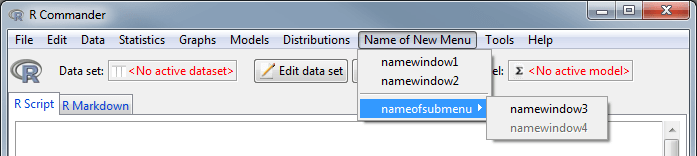
\includegraphics[width=12cm]{figures/examplemenus.png}
\caption{Exame of Menu Creation \label{examplemenus}}
\end{figure}


\subsection{\texttt{.onAttach}}
\noindent In order for your package to be recognised by \texttt{Rcmdr} as a
plug-in, you will need to add the following \texttt{.onAttach} function to your
package (see Appendix).

\subsection{\texttt{DESCRIPTION} and \texttt{NAMESPACE} File}
In order to use templates of the \verb|REST| package in your own package, you
should import both \verb|Rcmdr| and \verb|REST| in the DESCRIPTION and
NAMESPACE File.\\
This comes down to adding \verb|Imports: Rcmdr, REST| to the former and
\verb|import(Rcmdr,REST)| to the latter.

\subsection{Active Data in \texttt{Rcmdr}}
There are many ways to load data in R Commander, from the R workspace, from a
text file, excel file, SAS, etc. The important thing to know is that the loaded
data will become the active dataset in \texttt{Rcmdr}. This active dataset will
always be of the dataframe class, so it could be possible you will need to
transform it to a matrix if your function requires this.

\begin{figure}[H]
\centering
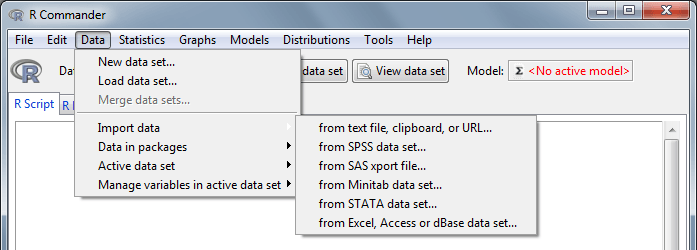
\includegraphics[width=9cm]{figures/rcmdr_datainput.png}
\caption{{\it R Commander - Data Menu}\label{datainput}}
\end{figure}
\begin{figure}[H]
\centering
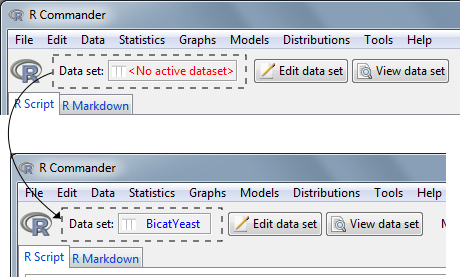
\includegraphics[width=9cm]{figures/rcmdr_activedataset.png}
\caption{{\it R Commander - Active Dataset}\label{activedataset}}
\end{figure}

\noindent {\it Short Summary:}
\begin{enumerate}
  \item \texttt{DESCRIPTION} and \texttt{NAMESPACE} file
  \item Add \texttt{.onAttach} function
  \item Create window functions with {\it template scripts}
  \item Add window functions to \texttt{menus.txt}
\end{enumerate}

\section{Script Templates Guide}

\subsection{General Script}
We will now start going through \texttt{general\_script.R} which can be found in
the appendix or the \verb|doc| folder of the \verb|REST| package.

\subsubsection{General Window Information}
\noindent The script starts by making a function which will be called on to
create a window. First thing you should do of course is to rename this function
to your own liking. Next, some objects (\verb|new.frames|, \verb|grid.config| and \verb|grid.rows|) are initialized that will be used to
store information about the window that you are about to create. 


\begin{knitrout}
\definecolor{shadecolor}{rgb}{0.969, 0.969, 0.969}\color{fgcolor}\begin{kframe}
\begin{alltt}
\hlstd{GUI_WINDOW} \hlkwb{<-} \hlkwa{function}\hlstd{(}\hlkwc{list.info}\hlstd{=}\hlkwd{list}\hlstd{())\{}

        \hlcom{##########################}
        \hlcom{## PREAMBLE/INFORMATION ##}
        \hlcom{##########################}

        \hlstd{dialogtitle} \hlkwb{<-} \hlstr{"This is the title of the window"}

        \hlstd{usetabs} \hlkwb{<-} \hlnum{TRUE}
        \hlstd{tabnames} \hlkwb{<-} \hlkwd{c}\hlstd{(}\hlstr{"Tab 1"}\hlstd{,}\hlstr{"Tab 2"}\hlstd{,}\hlstr{"Tab 3"}\hlstd{)}
        \hlstd{helppage} \hlkwb{<-} \hlstr{"plot"}

        \hlcom{# Do not change these lines}
        \hlkwa{if}\hlstd{(usetabs)\{ntabs} \hlkwb{<-} \hlkwd{length}\hlstd{(tabnames)\}} \hlkwa{else} \hlstd{\{ntabs} \hlkwb{<-} \hlnum{1}\hlstd{\}}
        \hlstd{new.frames} \hlkwb{<-} \hlkwd{.initialize.new.frames}\hlstd{(ntabs)}
        \hlstd{grid.config} \hlkwb{<-} \hlkwd{.initialize.grid.config}\hlstd{(ntabs)}
        \hlstd{grid.rows} \hlkwb{<-} \hlkwd{.initialize.grid.rows}\hlstd{(ntabs)}
        \hlcom{### end of "Do not change these lines"}

        \hlcom{##################}
        \hlcom{## GRID BUTTONS ##}
        \hlcom{##################}

        \hlstd{make.help.button} \hlkwb{<-} \hlnum{TRUE}
        \hlstd{make.setwd.button} \hlkwb{<-} \hlnum{TRUE}
        \hlstd{make.resetgws.button} \hlkwb{<-} \hlnum{TRUE}
        \hlstd{make.seed.button} \hlkwb{<-} \hlnum{TRUE}

        \hlcom{# ... continuation of the script down below (these 2 parts are put here)	}

\hlstd{\}}       \hlcom{# Note: The curly bracket is placed here for syntax reasons. }
        \hlcom{#       It should be placed after the call of GUI_template.}
\end{alltt}
\end{kframe}
\end{knitrout}
\noindent The scripts starts by filling in some information about your
new window. A clarifying example follows later in which we make a window of the
biclustering plaid method.
\begin{description}
  \item[$\bullet$ \texttt{dialogtitle}:] The title of the window which will be
  shown on top. (This can not be empty!)
  
  \item[$\bullet$ \texttt{usetabs}:] Logical value determining if tabs should be
  used.
  \item[$\bullet$ \texttt{tabnames}:] A vector containing names of the tabs if
  \verb|usetabs| is \verb|TRUE|. 
  
  \item[$\bullet$ \texttt{helppage}:] The name of the helppage the help button
  should be directed to. (\verb|help(helppage)|) This is only relevant if the
  help button is created in the grid.
\end{description}
\noindent After filling in these variables, you also have the possibility to add
some grid buttons. These are some standard buttons which will appear at the
bottom of your window or, if you are using multiple tabs, below all the tab
windows (Figure \ref{optionalgrid}). While the exit button will always be there,
you can add some additional ones by setting the following variables to
\verb|TRUE| or \verb|FALSE|. 
\begin{description}
  \item[$\bullet$ \texttt{make.help.button}:] A help button which leads to the
  help page defined by \verb|helppage|.
  \item[$\bullet$ \texttt{make.setwd.button}:] A button with which the user can
  change its working directory.
  \item[$\bullet$ \texttt{make.resetgws.button}:] A button with which the user
  can reset the global working space.
  \item[$\bullet$ \texttt{make.seed.button}:] Adds an entry field and button to
  set a certain seed.
\end{description}
\begin{figure}[H]
\centering
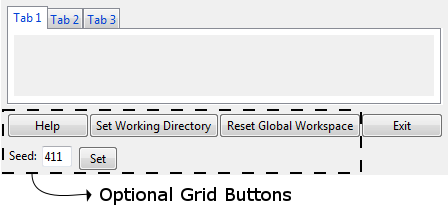
\includegraphics[width=9cm]{figures/optionalgrid.png}
\caption{Optional Grid Buttons \label{optionalgrid}}
\end{figure}

\noindent Before going on to the next part of the script, a short explanation
about \verb|list.info| (parameter of \verb|GUI_WINDOW| function) might be in
order. You do not necessarily have to use this, but it can bring a bit more
flexibility to your windows. This is especially the case when you are calling
a window from another window.\\
For example, let's say you have created a dialog for a certain graph called
\verb|graph_window|. You have not added it to the menu, but the function is
linked to a button in another window which will call \verb|method1_window|. You
however know that this graphing might also be interesting for method 2 so you
also link it to a button in \verb|method2_window|. Your goal now is for the
graph window to have a different dialog title, depending from which window it
was called from. You can achieve this by storing this information in
\verb|list.info|. \\
You could then use 
\verb|dialogtitle <- paste("Graph of ",list.info[[1]],sep="")| so that when you
call \verb|GRAPH_WINDOW(list(name="Method 1"))| from the button in the method 1
window, the title will reflect this ("Graph of Method 1").\\
This is of course a very simplistic example, but you can use this for all of the
variables in the script, creating very different windows depending on which
information is stored in \verb|list.info| (e.g. different frames, different
naming, etc.).

\subsubsection{Making a Tab}
After providing the information about the window we can finally start making
it! You can make as many tabs as you want, but they are all created in the same
three easy steps as shown in Figure \ref{3steps}:
\begin{enumerate}
\item Making the frames
\item Configuring the frames into a grid
\item Combining rows into a box
\end{enumerate}

\begin{figure}[H]
\centering
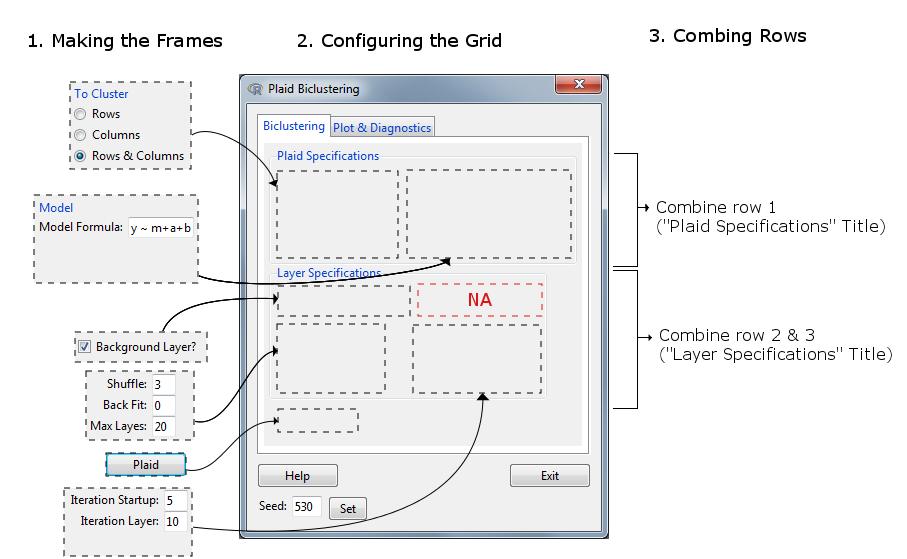
\includegraphics[width=\linewidth]{figures/3steps.png}
\caption{{\it Making windows in 3 steps}
\label{3steps}}
\end{figure}

\begin{knitrout}
\definecolor{shadecolor}{rgb}{0.969, 0.969, 0.969}\color{fgcolor}\begin{kframe}
\begin{alltt}
\hlcom{###########}
\hlcom{## TAB 1 ##}
\hlcom{###########}
\hlstd{Tab} \hlkwb{<-} \hlnum{1}

\hlcom{### 1. ADDING THE FRAMES ###}

\hlcom{# Add frames here}


\hlcom{### 2. CONFIGURING THE GRID ###}
\hlstd{grid.config} \hlkwb{<-} \hlkwd{.grid.matrix}\hlstd{(}\hlkwc{Tab}\hlstd{=Tab,}\hlkwd{c}\hlstd{(}\hlstr{"frame1"}\hlstd{,}\hlstr{"frame2"}\hlstd{,}\hlstr{"frame3"}\hlstd{,}\hlnum{NA}\hlstd{),}
                \hlkwc{byrow}\hlstd{=}\hlnum{TRUE}\hlstd{,}\hlkwc{nrow}\hlstd{=}\hlnum{2}\hlstd{,}\hlkwc{ncol}\hlstd{=}\hlnum{2}\hlstd{,}\hlkwc{grid.config}\hlstd{=grid.config)}


\hlcom{### 3. COMBINING THE ROWS ###}
\hlstd{grid.rows} \hlkwb{<-} \hlkwd{.combine.rows}\hlstd{(}\hlkwc{Tab}\hlstd{=Tab,}\hlkwc{rows}\hlstd{=}\hlkwd{c}\hlstd{(}\hlnum{1}\hlstd{,}\hlnum{2}\hlstd{),}\hlkwc{title}\hlstd{=}\hlstr{"A nice box: "}\hlstd{,}
                \hlkwc{border}\hlstd{=}\hlnum{TRUE}\hlstd{,}\hlkwc{grid.rows}\hlstd{=grid.rows,}\hlkwc{grid.config}\hlstd{=grid.config)}
\end{alltt}
\end{kframe}
\end{knitrout}
\noindent Looking at the script, you can see it starts with putting the
\verb|Tab| to $1$. This will make sure everything you are
creating and saving now will be done for the first tab. \\ \\
{\it Step 1:}\\
As already explained earlier, the first step will be to create the frames in
which you want to put your function arguments. A variety of frames can be
created, but these will be explained in more detail in the following section. To
give a quick summary, here is the list of the types of frames which can be
generated.
\begin{itemize}
  \item Check Boxes
  \item Radio Buttons
  \item Entry Fields
  \item Sliders
  \item Spinboxes
  \item List Box
  \item Manual Button
\end{itemize}
\noindent In future updates, there is still the possibility to add even more
types if required.
\\ \\
{\it Step 2:}\\
During the creation of the frames in the previous step, you will have given each
of them a unique name. Using these framenames, the next step will be to simply
order them into a matrix grid, filling in the empty spots with \verb|NA|'s.
This is achieved with the \verb|.grid.matrix| function. The function accepts
the exact same arguments as the \verb|matrix| function apart from two new ones,
namely \verb|Tab| and \verb|grid.config|. The first is to make sure the
template function knows we are adding frames in the first tab, while second one
is there to ensure that the new information is added to the old
\verb|grid.config| object and that old information is not lost.\\
Further, it is important to know that the inserted frames will {\it always} be
pulled towards the north-west as much as possible. Therefore in a 1-row
matrix, something like \verb|c(NA,"frame1")| or \verb|c("frame1",NA)| would give
exactly the same result.
\\ \\
{\it Step 3:}\\
The final step will enable you to put one or multiple rows in a seperate box
which can serve two different purposes. The first, being the most obvious one, is
simply to add some visual distinction between rows with the help of a title.
This can be with or without a border around the row(s).\\
The second purpose is connected to the way frames are added in this {\it grid}.
Sometimes if frames have a large difference in size, other frames might seem to
be jumping to the right, trying to fit in one general grid. In general if you
see this happening, putting this row(s) in a box will solve this problem and the
frames will again be pulled towards the left.\\
Creating these boxes by combining rows is again very easy, one simply needs to
use the \verb|.combine.rows| function which will save the necessary information
in the \verb|grid.rows| object. The function only has three arguments you should
change: \verb|rows| which is a vector containing the rows you wish to
combine, \verb|title| to give the box a title (\verb|""| means no title) and
\verb|border| to decide if there should be a border.\\
Note that in contrast to the grid configuration, you can call this function
multiple times until the desired result is obtained.
\begin{knitrout}
\definecolor{shadecolor}{rgb}{0.969, 0.969, 0.969}\color{fgcolor}\begin{kframe}
\begin{alltt}
\hlcom{#############}
\hlcom{### TAB 2 ###}
\hlcom{#############}
\hlstd{Tab} \hlkwb{<-} \hlnum{2}

\hlcom{# Repeat the 3 steps of tab 1 for as many tabs as you like...}


\hlcom{###################################################################}
\hlcom{## USE ALL THE ARGUMENTS IN THE GENERAL GUI_TEMPLATE FUNCTION    ##}
\hlcom{###################################################################}
\hlkwd{GUI_template}\hlstd{(}\hlkwc{dialogtitle}\hlstd{=dialogtitle,}\hlkwc{helppage}\hlstd{=helppage,}\hlkwc{make.resetgws.button}\hlstd{=}
                \hlstd{make.resetgws.button,}\hlkwc{make.setwd.button}\hlstd{=make.setwd.button,}
                \hlkwc{make.help.button}\hlstd{=make.help.button,}\hlkwc{make.seed.button}\hlstd{=make.seed.button,}
                \hlkwc{usetabs}\hlstd{=usetabs,}\hlkwc{tabnames}\hlstd{=tabnames,}\hlkwc{grid.config}\hlstd{=grid.config,}\hlkwc{grid.rows}\hlstd{=grid.rows,}
                \hlkwc{new.frames}\hlstd{=new.frames)}
\end{alltt}
\end{kframe}
\end{knitrout}
\noindent Next, you can repeat these 3 steps for as many tabs as you have
defined in the beginning. Finally, to end the \verb|GUI_WINDOW| function, the
\verb|GUI_template| function is called with all of your defined variables. 
This is our automated template function we created in the \verb|REST| package in
order to complete the window creation. This means that this function will be responsible
for actually creating your window.

\subsection{Frame Scripts}
In this section, the several types of frames which can be used in the
\verb|general_script| will be showcased. The idea is that these parts of the
R-code (which are also in the Appendix) are copy-pasted into the
\verb|general_script| and are adjusted as deemed necessary. \\
All the frame types have the \verb|title| and
\verb|border| option in common. The results of these options can be seen in
Figure \ref{titleborder}. Also note that for each frametype the information is
saved in one object, namely \verb|new.frames|. Just as the grid and row configuration
earlier, new information will keep on getting added to this object, now with
the help of the \verb|.add.frame| function. Lastly, at the start of each frame
script, a \verb|type| variable will be set to determine the type of frame for
this previous mentioned \verb|.add.frame| function.

\begin{figure}[H]
\centering
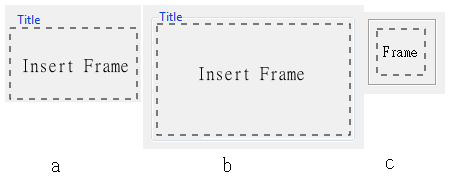
\includegraphics[scale=0.8]{figures/title_border.png}
\caption{{\bf A.}{\it Title and No Border} {\bf B.}{\it Title and Border} {\bf
C.}{\it No Title and Border}
\label{titleborder}}
\end{figure}


\noindent {\bf Entry Fields}\\
\noindent The first type of frame is the entry fields frame. It can be used for
both numerical arguments and character arguments of your function tied to a
button. Multiple entries can be added in one frame which will be placed below
each other.
\begin{figure}[H]
\centering
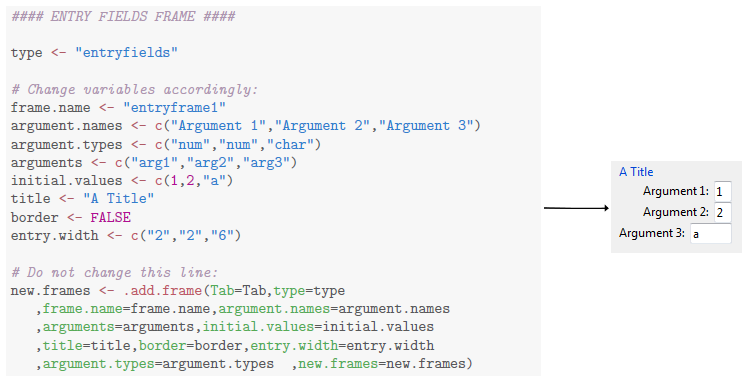
\includegraphics[scale=0.5]{figures/entryfields.png}
\caption{{\it Entry Fields: Code + Example}
\label{entryfields}}
\end{figure}

\noindent {\it Entry Fields Variables:}
\begin{description}
  \item[$\bullet$ \texttt{frame.name}:] The unique name of this frame. (Which is used in the grid matrix)
  \item[$\bullet$ \texttt{argument.names}:] The argument names how they will
  appear in the window.
  \item[$\bullet$ \texttt{argument.types}:] A vector defining if the argument is
  \verb|"num"| or \verb|"char"|. This basically just means if there should be a
  \verb|' '| around the value when filling it in in the function. (e.g. In
  Figure \ref{entryfields} the arguments would be filled in as \verb|,arg1=1,arg2=2,arg3='a'|)
  \item[$\bullet$ \texttt{arguments}:] The actual argument names, used for the
  function. Note it is not necessary for these to be unique between multiple
  frames.
  \item[$\bullet$ \texttt{initial.values}:] A vector containing the initial
  values in the entry fields.
  \item[$\bullet$ \texttt{title}:] Optional title for the frame (\verb|""| means no title)
  \item[$\bullet$ \texttt{border}:] Logical value determining the presence of a
  border.
  \item[$\bullet$ \texttt{entry.width}:] A vector containing the width of the
  entry fields (1 width = 1 number/character).
\end{description}

%\vspace{0.5cm}
\noindent {\bf Check Boxes}\\
The second type of frame is the check boxes frame which is used for
\verb|TRUE|/\verb|FALSE| arguments. Just like for entry fields, multiple check
boxes can be added below each other. 
\begin{figure}[H]
\centering
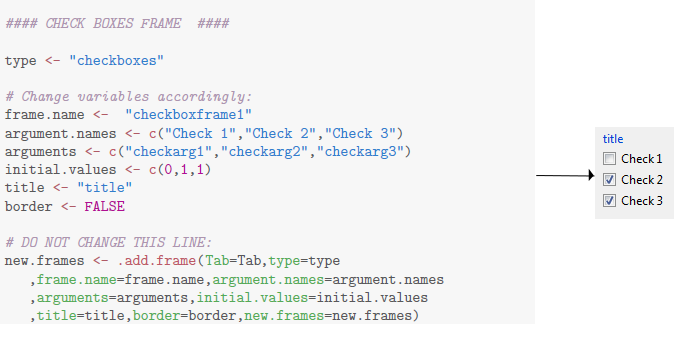
\includegraphics[scale=0.5]{figures/checkboxes.png}
\caption{{\it Check Boxes: Code + Example}
\label{checkboxes}}
\end{figure}

\noindent {\it Check Boxes Variables:}
\begin{description}
  \item[$\bullet$ \texttt{frame.name}:] The unique name of this frame. (Which is used in the grid matrix)
  \item[$\bullet$ \texttt{argument.names}:] The argument names how they will
  appear in the window.
  \item[$\bullet$ \texttt{arguments}:] The actual argument names, used for the
  function. Note it is not necessary for these to be unique between multiple
  frames.
  \item[$\bullet$ \texttt{initial.values}:] A vector containing the initial
  values in the entry fields. (0 for \verb|FALSE|, 1 for \verb|TRUE|)
  \item[$\bullet$ \texttt{title}:] Optional title for the frame (\verb|""| means no title)
  \item[$\bullet$ \texttt{border}:] Logical value determining the presence of a
  border. 
\end{description}


\noindent {\bf Radio Buttons}\\
The next type is radio buttons, which is used for only one argument with a
finite number of values.
\begin{figure}[H]
\centering
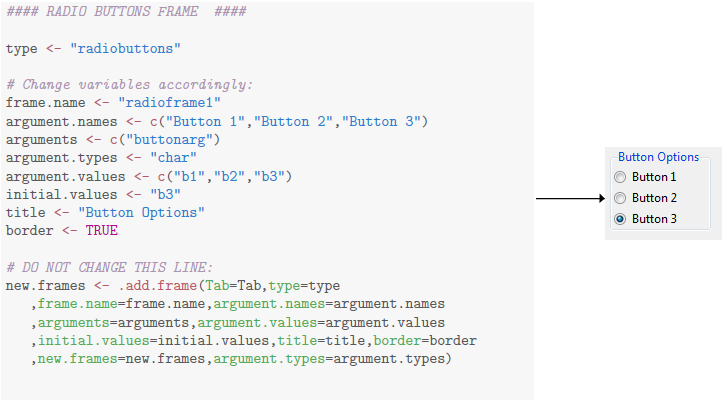
\includegraphics[scale=0.5]{figures/radiobuttons.png}
\caption{{\it Radio Buttons: Code + Example}
\label{radiobuttons}}
\end{figure}

\noindent {\it Radio Buttons Variables:}
\begin{description}
  \item[$\bullet$ \texttt{frame.name}:] The unique name of this frame. (Which is used in the grid matrix)
  \item[$\bullet$ \texttt{argument.names}:] The names of the buttons how they
  will appear in the window.
  \item[$\bullet$ \texttt{arguments}:] The actual argument name, used for the
  function. Note it is not necessary for these to be unique between multiple
  frames. (Only 1 argument!)
  \item[$\bullet$ \texttt{argument.types}:] Just as for the entry fields, this
  will determine of the values are filled in with or without \verb|' '|. The two
  options are again \verb|"num"| and \verb|"char"|, but in contrast with the entry
  fields it is now only one value and not a vector.
  \item[$\bullet$ \texttt{argument.values}:] The actual values of the radio buttons 
that correspond to the values passed to the function. 
    \item[$\bullet$ \texttt{initial.values}:] The initial value of the radio
  buttons. It will determine which button is selected on opening the window.
  \item[$\bullet$ \texttt{title}:] Optional title for the frame (\verb|""| means no title)
  \item[$\bullet$ \texttt{border}:] Logical value determining the presence of a
  border.   

\end{description}

\noindent {\bf Value Sliders}\\
The following type will create value sliders which can only be used for
numerical values. Again multiple sliders can be placed under each other. The
current value of the slider will always appear on top of it.

\begin{figure}[H]
\centering
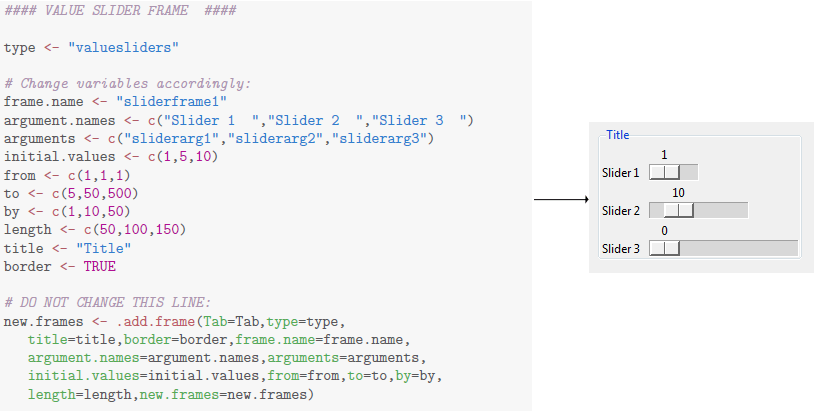
\includegraphics[scale=0.5]{figures/slider.png}
\caption{{\it Value Slider: Code + Example}
\label{radiobuttons}}
\end{figure}

\noindent {\it Value Sliders Variables:}
\begin{description}
  \item[$\bullet$ \texttt{frame.name}:] The unique name of this frame. (Which is used in the grid matrix)
  \item[$\bullet$ \texttt{argument.names}:] The argument names how they will
  appear in the window.  
  \item[$\bullet$ \texttt{arguments}:] The actual argument names, used for the
  function. Note it is not necessary for these to be unique between multiple
  frames.
  \item[$\bullet$ \texttt{initial.values}:] Vector of initial values of the
  sliders. Depending on the possible values the slider can take, this value will
  shift towards it (e.g. Slider 3: 10 as initial value but it was shifted to 0
  since this is the closest value the slider represent).
  \item[$\bullet$ \texttt{from}:] Vector of starting points of the slider
  (note: depending on the \verb|length|, \verb|to| and \verb|by| parameter, this
  `from' value could change slightly. It will choose the closest and most
  fitting value to display the slider properly. e.g. Slider 3 starts from 0
  instead of 1).
  \item[$\bullet$ \texttt{to}:] Vector of ending points of the sliders.
  \item[$\bullet$ \texttt{by}:] Vector with the values determining how one
  movement of the sliders will change the current value.
  \item[$\bullet$ \texttt{length}:] Vector containing the lengths of the
  sliders.
  \item[$\bullet$ \texttt{title}:] Optional title for the frame (\verb|""| means no title)
  \item[$\bullet$ \texttt{border}:] Logical value determining the presence of a
  border.   
  
\end{description}


\noindent {\bf Spin Boxes}\\
This type will create spin boxes which are again solely used for numerical
values. Just as for sliders, multiple spin boxes can be placed below each other.

\begin{figure}[H]
\centering
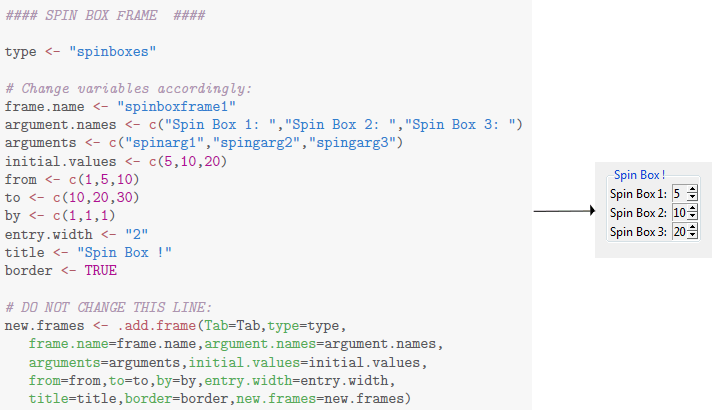
\includegraphics[scale=0.5]{figures/spinboxes.png}
\caption{{\it Spin Boxes: Code + Example}
\label{spinboxes}}
\end{figure}

\noindent {\it Spin Boxes Variables:}
\begin{description}
  \item[$\bullet$ \texttt{frame.name}:] The unique name of this frame. (Which is used in the grid matrix)
  \item[$\bullet$ \texttt{argument.names}:] The argument names how they will
  appear in the window.  
  \item[$\bullet$ \texttt{arguments}:] The actual argument names, used for the
  function. Note it is not necessary for these to be unique between multiple
  frames.
  \item[$\bullet$ \texttt{initial.values}:] Vector of initial values of the
  spin boxes.
  \item[$\bullet$ \texttt{from}:] Vector of starting points of the spin boxes.
  \item[$\bullet$ \texttt{to}:] Vector of ending points of the spin boxes.
  \item[$\bullet$ \texttt{by}:] Vector with the values determining how much one
  click will change the current value.
  \item[$\bullet$ \texttt{entry.width}:] Width of all the spinboxes (one value
  which applies to all of them)
  \item[$\bullet$ \texttt{title}:] Optional title for the frame (\verb|""| means no title)
  \item[$\bullet$ \texttt{border}:] Logical value determining the presence of a
  border.   
  
\end{description}

\noindent {\bf List Box}\\
\noindent The next type is called a list box. This box corresponds with 1
argument for which several values are available. With the list box it is possible to select
one or multiple from the box, putting them in a vector.
\begin{figure}[H]
\centering
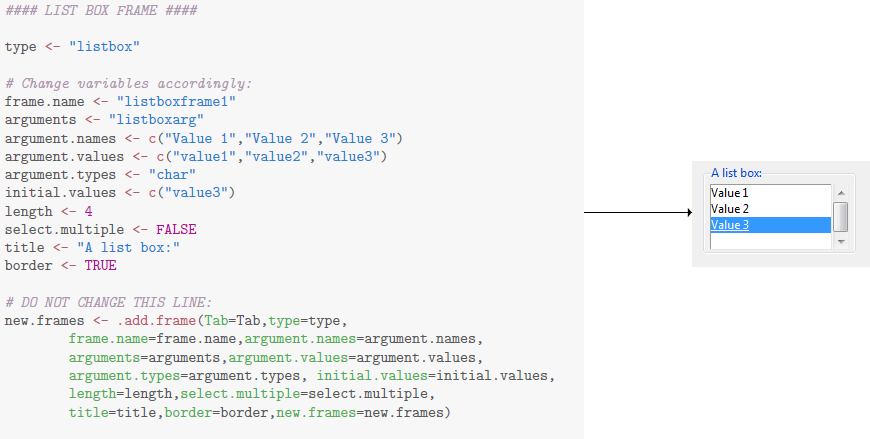
\includegraphics[scale=0.5]{figures/listbox.png}
\caption{{\it List Box: Code + Example}
\label{listbox}}
\end{figure}

\noindent {\it List Box Variables:}
\begin{description}
  \item[$\bullet$ \texttt{frame.name}:] The unique name of this frame. (Which is used in the grid matrix)
  \item[$\bullet$ \texttt{arguments}:] The actual argument name, used for the
  function. Note it is not necessary for these to be unique between multiple
  frames. (Only 1 argument!)
  \item[$\bullet$ \texttt{argument.names}:] The labels of the items how they
  will appear in the box.
  \item[$\bullet$ \texttt{argument.values}:] The actual values of the list items 
  that correspond to the values passed to the function. 
  \item[$\bullet$ \texttt{argument.types}:] Just as for the entry fields, this
  will determine of the values are filled in with or without \verb|' '|. The two options
  are again \verb|"num"| and \verb|"char"|, but in contrast with the entry
  fields it is now only one value and not a vector. (Same as for radio buttons)
  \item[$\bullet$ \texttt{initial.values}:] The initial value of the list box.
  It will determine which list item is selected on opening the window.
  \item[$\bullet$ \texttt{length}:] A value corresponding with the height of the
  box. (If no value or \verb|c()| is given, the length of the
  \verb|argument.names| will be used)
  \item[$\bullet$ \texttt{select.multiple}:] A logical value determining if it
  should be possible selecting only 1 or multiple list items. For example if the
  \verb|argument.types| would be \verb|"char"| and \verb|select.multiple| would
  be \verb|FALSE|, then an example would be simply \verb|'value1'|. If the
  latter would have been \verb|TRUE|, the result would look like
  \verb|c('value1','value3')|. (In the case those were selected)
  \item[$\bullet$ \texttt{title}:] Optional title for the frame (\verb|""| means
  no title)
  \item[$\bullet$ \texttt{border}:] Logical value determining the presence of a
  border.   
\end{description}


\noindent {\bf Manual Buttons}\\
The last type of frame which can be utilized, is making manual buttons. There
are two primary uses for these buttons. The first use is to simple execute a
function, based on the arguments of other frames in the window. The second
application is to tie the button to another window function to open up more options.

\begin{figure}[H]
\centering
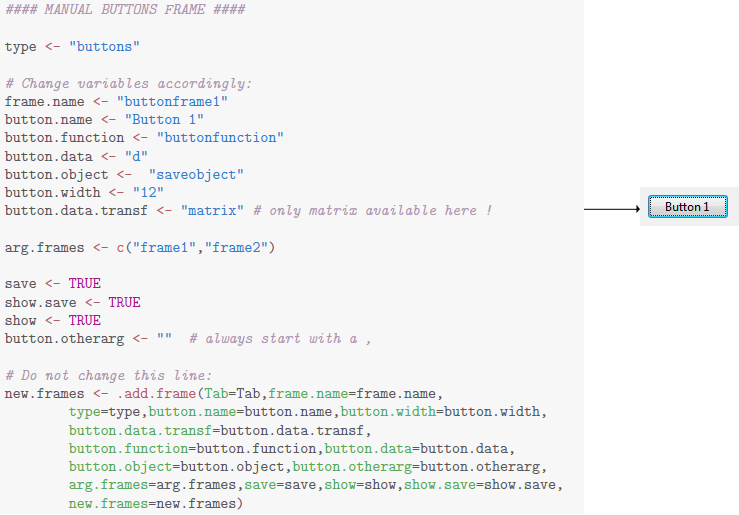
\includegraphics[scale=0.5]{figures/manualbutton.png}
\caption{{\it Manual Button: Code + Example}
\label{manualbutton}}
\end{figure}

\noindent {\it Manual Button Variables:}
\begin{description}
  \item[$\bullet$ \texttt{frame.name}:] The unique name of this frame. (Which is used in the grid matrix)
  \item[$\bullet$ \texttt{button.name}:] The text which will appear on the
  button. 
  \item[$\bullet$ \texttt{button.function}:] A string of the name of the
  function which should be tied to this button. Another useful practice is to actually make an entire
  new function for this manual button. This new function could then for
  example contain a series of functions which would then be carried
  out all at the same time when clicking on this button.
  \item[$\bullet$ \texttt{button.data}:] The name of the data argument the
  button function. The data which is loaded in R Commander will then be
  pasted after this argument. (Simply put \verb|""| when this is not necessary)
  \item[$\bullet$ \texttt{button.object}:] If it is chosen to save what is
  returned by \verb|button.function|, it will saved in an object with the name
  given here.
  \item[$\bullet$ \texttt{button.width}:] Character containing the width of the
  button. (Default = \verb|"12"|)
  \item[$\bullet$ \texttt{button.data.transf}:] Character determining if the
  data for \verb|button.data| should be transformed. (Only \verb|"matrix"| is
  possible at this time)
  \item[$\bullet$ \texttt{button.otherarg}:] A string containing extra arguments you
  do {\it not} want the user to change. For example if a button was tied to the
  \verb|sum| function, but you want to always remove the \verb|NA|'s without the
  user interference. Then \verb|button.otherarg| should be equal to
  \verb|",na.rm=TRUE"|. This means that for this button this part of the
  arguments will always be added. (Since these are extra arguments being added,
  note that a comma should always be used in the beginning. Of course you are
  also not limited to adding only 1 extra arguments, you can add as many as
  necessary. (\verb|",arg1=1 ,arg2=10"|) Simply add them here as you would add
  them inside the function itself.)
  \item[$\bullet$ \texttt{arg.frames}:] A vector containing the names of those
  frames from which this button function should pull its arguments.
  \item[$\bullet$ \texttt{save}:] Logical value determining if the result of the
  button function should be saved. For example for a plotting function this is
  mosty likely not necessary, however for a diagnostic result it is. The
  difference between a \verb|TRUE| and \verb|FALSE| option is shown in figure
  \ref{manualbutton_showsave}.
  \item[$\bullet$ \texttt{show.save}:] Logical value determining if the saved
  result should be printed afterwards as well. (See Figure \ref{manualbutton_showsave})
  \item[$\bullet$ \texttt{show}:] Logical value determining if the button
  function should be shown in R Commander. It is good practice to do this for
  the plotting and diagnostics functions however if is a function to create a
  new window, it is probably not necessary to show it. (See Section
  \ref{sec:doitandprint} for another use.)

\end{description}


\begin{figure}[H]
\centering
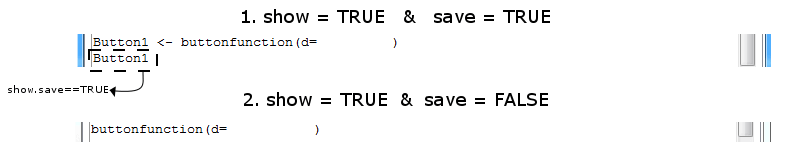
\includegraphics[scale=0.5]{figures/manualbutton_showsave.png}
\caption{{\it Manual Buttons - save option}
\label{manualbutton_showsave}}
\end{figure}

\subsection{Example Script - Plaid Biclustering}
In this small section, we will demonstrate some parts of window creation in an
example. The example which was chosen was to implement a biclustering method,
namely the {\it Plaid} method. (The full code can be found in the Appendix)


\begin{knitrout}
\definecolor{shadecolor}{rgb}{0.969, 0.969, 0.969}\color{fgcolor}\begin{kframe}
\begin{alltt}
\hlstd{plaid_WINDOW} \hlkwb{<-} \hlkwa{function}\hlstd{(}\hlkwc{list.info}\hlstd{=}\hlkwd{list}\hlstd{())\{}

    \hlcom{##########################}
    \hlcom{## PREAMBLE/INFORMATION ##}
    \hlcom{##########################}

    \hlstd{dialogtitle} \hlkwb{<-} \hlstr{"Plaid Biclustering"}

    \hlstd{usetabs} \hlkwb{<-} \hlnum{TRUE}
    \hlstd{tabnames} \hlkwb{<-} \hlkwd{c}\hlstd{(}\hlstr{"Biclustering"}\hlstd{,}\hlstr{"Plot & Diagnostics"}\hlstd{)}

    \hlkwa{if}\hlstd{(usetabs)\{ntabs} \hlkwb{<-} \hlkwd{length}\hlstd{(tabnames)\}} \hlkwa{else} \hlstd{\{ntabs} \hlkwb{<-} \hlnum{1}\hlstd{\}}
    \hlstd{new.frames} \hlkwb{<-} \hlkwd{.initialize.new.frames}\hlstd{(ntabs)}
    \hlstd{grid.config} \hlkwb{<-} \hlkwd{.initialize.grid.config}\hlstd{(ntabs)}
    \hlstd{grid.rows} \hlkwb{<-} \hlkwd{.initialize.grid.rows}\hlstd{(ntabs)}

    \hlstd{helppage} \hlkwb{<-} \hlstr{"BCPlaid"}

    \hlcom{##################}
    \hlcom{## GRID BUTTONS ##}
    \hlcom{##################}

    \hlstd{make.help.button} \hlkwb{<-} \hlnum{TRUE}
    \hlstd{make.setwd.button} \hlkwb{<-} \hlnum{FALSE}
    \hlstd{make.resetgws.button} \hlkwb{<-} \hlnum{FALSE}
    \hlstd{make.seed.button} \hlkwb{<-} \hlnum{TRUE}

        \hlcom{#... followed by tabs, frames,...}
\hlstd{\}}
\end{alltt}
\end{kframe}
\end{knitrout}
\noindent First of all the general information is filled out in the script
above.
This dialog contains two tabs with a help and seed grid button. 
The code for the second tab has been omitted in the Appendix.\\
Next in Figure \ref{plaidbuilding}, some of the frames are highlighted with
their corresponding code. Note also the use of the buttons and how frames are
chosen to give the arguments to the function tied to the button (red arrows).\\
The function used to execute the plaid algorithm is called \verb|biclust| with
the argument \verb|method=BCPlaid()|. The latter you can see coming back in the
\verb|button.otherarg|. This means the end result would look something like
\begin{verbatim}
PlaidResult <- biclust(x=data,method=BCPlaid(),background=TRUE,
                                shuffle=3,back.fit=0,max.layers=20,...)
\end{verbatim}
with of course the extra addition of the other parameters of other frames (the
frames defined in \verb|arg.frames|).

\begin{figure}[H]
\centering
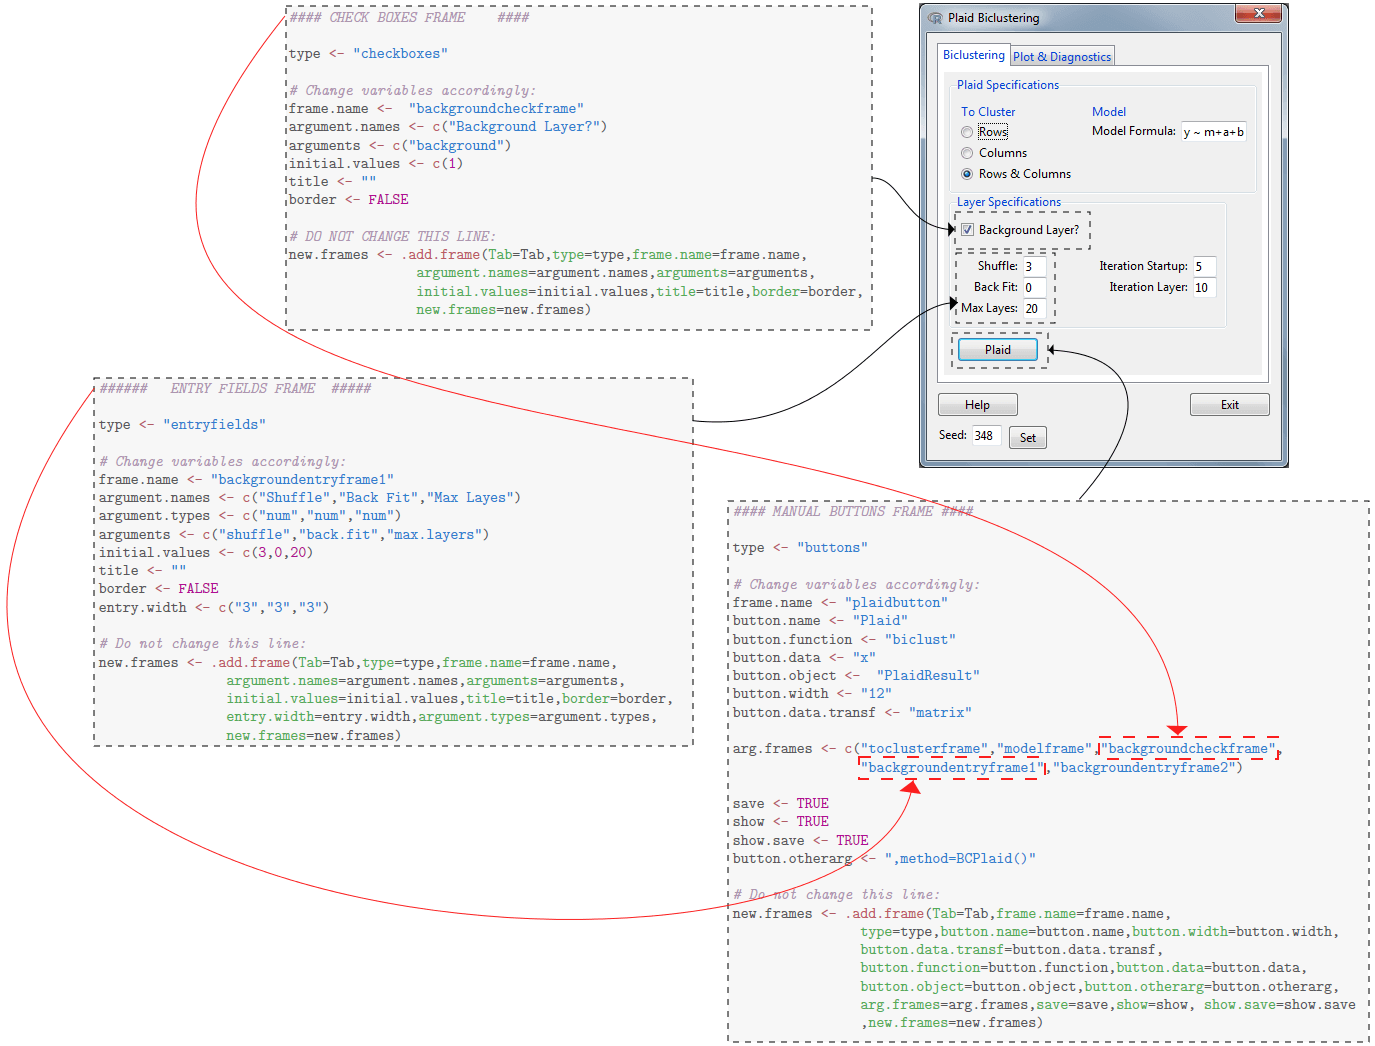
\includegraphics[width=\linewidth]{figures/plaidbuilding.png}
\caption{Building the Plaid Window \label{plaidbuilding}}
\end{figure}
\noindent Following the rest of the frame creations is of course the grid
configuring and the row combining of the first tab. In this extract of the
script, one can see the frames from Figure \ref{plaidbuilding} being
placed in the last three of the four rows of the matrix after which the second
and third row are made into a box with border and {\it Layer Specifications} title.

\begin{knitrout}
\definecolor{shadecolor}{rgb}{0.969, 0.969, 0.969}\color{fgcolor}\begin{kframe}
\begin{alltt}
\hlcom{### 2. CONFIGURING THE GRID ###}
\hlstd{grid.config} \hlkwb{<-} \hlkwd{.grid.matrix}\hlstd{(}\hlkwc{Tab}\hlstd{=Tab,}\hlkwd{c}\hlstd{(}\hlstr{"toclusterframe"}\hlstd{,}\hlstr{"modelframe"}\hlstd{,}\hlstr{"backgroundcheckframe"}
                \hlstd{,}\hlnum{NA}\hlstd{,}\hlstr{"backgroundentryframe1"}\hlstd{,}\hlstr{"backgroundentryframe2"}\hlstd{,}\hlstr{"plaidbutton"}\hlstd{,}\hlnum{NA}\hlstd{),}
                \hlkwc{byrow}\hlstd{=}\hlnum{TRUE}\hlstd{,}\hlkwc{nrow}\hlstd{=}\hlnum{4}\hlstd{,}\hlkwc{ncol}\hlstd{=}\hlnum{2}\hlstd{,}\hlkwc{grid.config}\hlstd{=grid.config)}


\hlcom{### 3. COMBINING THE ROWS ###}
\hlstd{grid.rows} \hlkwb{<-} \hlkwd{.combine.rows}\hlstd{(}\hlkwc{Tab}\hlstd{=Tab,}\hlkwc{rows}\hlstd{=}\hlkwd{c}\hlstd{(}\hlnum{1}\hlstd{),}\hlkwc{title}\hlstd{=}\hlstr{"Plaid Specifications"}\hlstd{,}\hlkwc{border}\hlstd{=}\hlnum{TRUE}\hlstd{,}
                \hlkwc{grid.rows}\hlstd{=grid.rows,}\hlkwc{grid.config}\hlstd{=grid.config)}
\hlstd{grid.rows} \hlkwb{<-} \hlkwd{.combine.rows}\hlstd{(}\hlkwc{Tab}\hlstd{=Tab,}\hlkwc{rows}\hlstd{=}\hlkwd{c}\hlstd{(}\hlnum{2}\hlstd{,}\hlnum{3}\hlstd{),}\hlkwc{title}\hlstd{=}\hlstr{"Layer Specifications"}\hlstd{,}\hlkwc{border}\hlstd{=}\hlnum{TRUE}\hlstd{,}
                \hlkwc{grid.rows}\hlstd{=grid.rows,}\hlkwc{grid.config}\hlstd{=grid.config)}


\hlcom{#### Plot & Diagnostics Tab has been omitted ###}


\hlcom{###################################################################}
\hlcom{## USE ALL THE ARGUMENTS IN THE GENERAL GUI_TEMPLATE FUNCTION    ##}
\hlcom{###################################################################}
\hlkwd{GUI_template}\hlstd{(}\hlkwc{dialogtitle}\hlstd{=dialogtitle,}\hlkwc{helppage}\hlstd{=helppage,}\hlkwc{make.resetgws.button}\hlstd{=}
        \hlstd{make.resetgws.button,}\hlkwc{make.setwd.button}\hlstd{=make.setwd.button,}\hlkwc{make.help.button}\hlstd{=}
        \hlstd{make.help.button,}\hlkwc{make.seed.button}\hlstd{=make.seed.button,}\hlkwc{usetabs}\hlstd{=usetabs,}\hlkwc{tabnames}\hlstd{=}
        \hlstd{tabnames,}\hlkwc{grid.config}\hlstd{=grid.config,}\hlkwc{grid.rows}\hlstd{=grid.rows,}\hlkwc{new.frames}\hlstd{=new.frames)}
\end{alltt}
\end{kframe}
\end{knitrout}
\noindent Finally, the \verb|GUI_template| function is used to combine all the
gathered information and create the actual window.
\subsection{Testing your windows}
To test your created window function, first load in the \texttt{REST} package
which will launch the basic R Commander interface. Now open up an empty script
and paste your window script there. Going back to the example in the previous
section, this would simply mean pasting the entire \verb|plaid_WINDOW| function
here. Now run this function in R and your new window will appear on top
of the R Commander Interface.\\
If necessary, load in some data first before you start testing out the buttons
and checking if the right functions are appearing in the R Commander window.


\subsection{Advanced Techniques}
\subsubsection{Using \texttt{doItAndPrint()} and \texttt{justDoIt()}}
\label{sec:doitandprint}
We have seen before that for {\it manual buttons}, there is a variable called
\verb|show| which will prevent the function from being printed in R Commander.
This is helpfull if this function is simply to open up a new window. There is
however another way you can use this option (\verb|show==FALSE|) in combination
with \verb|save==FALSE|. \\
In this case, nothing is shown and nothing is saved when you click the button.
The function tied to the button is simply being executed. What will be shown now
is how to let several functions appear in the R-Commander screen instead of only
one.\\
This is done through the help of the following two \verb|Rcmdr| functions. In
these functions the \verb|command| argument is simply an R-expression in
character format. (e.g. \verb|"a <- 10+9"| or \verb|"b <- mean(c(1,2,3,4))"| or \verb|"a+b"|)
\begin{description}
  \item[$\bullet$ \texttt{doItAndPrint(command)}:] This function will print the
  command to the script window and execute.
  \item[$\bullet$ \texttt{justDoIt(command)}:] This fucntion will only execute
  the command in the output window, but not print it in the script window.
\end{description}

\noindent So for example what you could do is make a function containing these
\verb|doItAndPrint| and/or \verb|justDoIt|, and then link it to a button. Like
this you can send multiple commands (containing functions, expressions,...) to
the R Commander windows by clicking only a single button in your GUI.
\\ \\
{\bf Tips:}
\begin{enumerate}
\item Use \verb|paste()| or \verb|paste0()| for the creation of your
commands. By using these functions you can let your commands be created by the
arguments of the function linked to the button.
\item If you need to use characters in a command, use \verb|' '| or \verb|\" \"|.\\
(e.g. \verb|command <- paste0("names <- c('one','two')")| \\
or \verb|command <- paste0("names <- c(\"one\",\"two\")")|)
\item \verb|ActiveDataSet()| will give back the name of the current active dataset in
R Commander.
\end{enumerate}

\noindent {\it Example:}\\
In this example \verb|CenterColumns| is linked to a button and will compute
either the medians or the means of the columns of the active dataset (which is a
data frame) and then plot these. Note that the function has an argument which it will receive to
either use the median or mean.

\begin{knitrout}
\definecolor{shadecolor}{rgb}{0.969, 0.969, 0.969}\color{fgcolor}\begin{kframe}
\begin{alltt}
\hlstd{CenterColumns} \hlkwb{<-} \hlkwa{function}\hlstd{(}\hlkwc{type}\hlstd{=}\hlkwd{c}\hlstd{(}\hlstr{"mean"}\hlstd{,}\hlstr{"median"}\hlstd{))\{}
        \hlstd{command} \hlkwb{<-} \hlkwd{paste0}\hlstd{(}\hlstr{"center.vector <- apply("}\hlstd{,}\hlkwd{ActiveDataSet}\hlstd{(),}
                                       \hlstr{",MARGIN=2,FUN="}\hlstd{,type,}\hlstr{")"}\hlstd{)}
        \hlkwd{doItAndPrint}\hlstd{(command)}
        \hlkwd{doItAndPrint}\hlstd{(}\hlstr{"center.vector"}\hlstd{)}

        \hlkwd{doItAndPrint}\hlstd{(}\hlkwd{paste0}\hlstd{(}\hlstr{"plot(center.vector,main='Column Centers',xlab='Columns',
                               ylab='Value')"}\hlstd{))}
\hlstd{\}}
\end{alltt}
\end{kframe}
\end{knitrout}
\noindent Clicking this button with mean as an argument would then result in
Figure \ref{doitandprint_example}, accompanied by the plot in a graphics device.
\begin{figure}[H]
\centering
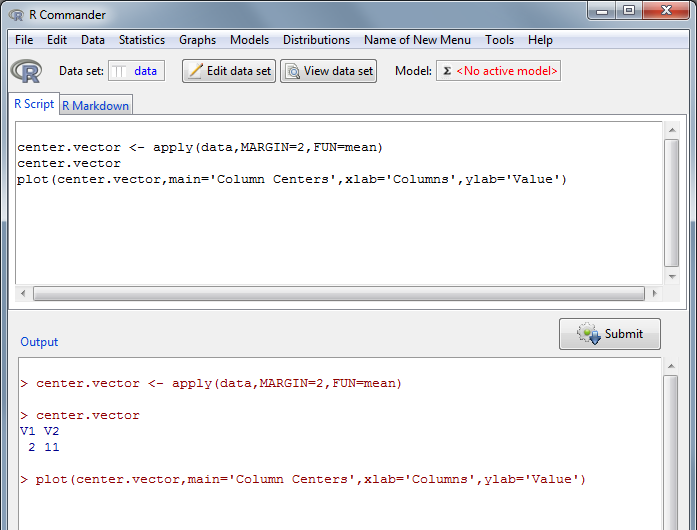
\includegraphics[width=12cm]{figures/doitandprint_example.png}
\caption{Example - CenterColumns \label{doitandprint_example}}
\end{figure}


\subsubsection{Window Environments}
\noindent When a window is being created, all the variables (such as
\verb|new.frames|) are being saved in a certain environment. You could see this
as a box in which all the parameters and variables connected with this window
reside. By using the \verb|GetWindowsENVIR()| function, you will get back a
\verb|list| object of which each element corresponds to a window which has
been used. The name of such a list element is the \verb|dialogtitle| and the
element itself is the created environment. Also remember that each time you
reopen a window, the environment will change to a new one and if you call the
\verb|list| object again, this change will be visible here too.\\
Now you might wonder why knowing this environment could be useful. By having
access to these variables of another window, you can change these at any time,
giving your GUI even more flexibility.\\
An easy example could be that you have a button called {\it `Presets'} on your
main window. Pressing this button would then open up a new window in which the
user can select with a radio button which one of the presets it would like
(Preset 1, Preset 2,...). In this new window the user could then click on an
{\it OK} button. The function tied to this button would then, with the above
described process, change all the inputs in the main window (to this preset) before closing down
the second window.
\\
While this can be done manually, to facilitate this process, some functions were
created for the most used application, namely changing what the user can enter
in the GUI. Also an example will be given for clarification.
\\ \\
{\bf \underline{Functions}}
\\ \\
\noindent \verb|ChangeWindow(dialogtitle, tab=1, framename, argument, new.value)|
\\ \\
\noindent {\it Description:}\\
\noindent This function will change the value the user can choose/enter in the
frames. The behaviour is a bit different for the types of frames. See
\verb|new.value| for more details.
\begin{description}
  \item[$\bullet$ \texttt{dialogtitle}:] The title of window which is going to
  be altered. This should be the same as \verb|dialogtitle| in your window
  script.
  \item[$\bullet$ \texttt{tab}:] The number of the tab in which you want
  something changed (if no tabs are used, choose number 1).
  \item[$\bullet$ \texttt{framename}:] The name of the frame in which something
  is going to be changed (same name as in the window script).
  \item[$\bullet$ \texttt{argument}:] The name of the argument in which
  something should be changed (same as in the window script).
  \item[$\bullet$ \texttt{new.value}:] The new value which should be entered for
  this argument in this particular frame. \verb|new.value| should almost always
  be a character (string), unless you are using it to change something in a list
  box.
  \begin{description}
    \item[$\triangleright$ {\it Entry Fields:}] \verb|new.value| should be a
    character/string (can be anything) which will then be pasted in entry field
    of the chosen argument. (e.g. \verb|"5"|, \verb|"c(1,2,3)"| or \verb|"c('one','two')"|)
    \item[$\triangleright$ {\it Check Boxes:}] \verb|new.value| should be
    either \verb|"0"| or \verb|"1"| which corresponds with unchecked and
    checked.
    \item[$\triangleright$ {\it Radio Buttons:}] \verb|new.values| should be
    that one of the \verb|argument.values| you wish to be selected
    \item[$\triangleright$ {\it Value Sliders:}] \verb|new.values| should be a
    character containing the numerical value you want the slider to be on (e.g.
    \verb|"10"|). Note that this value will be rounded to the closest possible
    position on the slider.
    \item[$\triangleright$ {\it Spin Boxes:}] \verb|new.values| should be a
    character containing the numerical value you want to spinbox to have (e.g.
    \verb|"5"|). Note that this value will be rounded to one of the possible
    values the spin box can take.
    \item[$\triangleright$ {\it List Box:}] Instead of simply changing which
    items are selected in the box, \verb|new.values| will instead change the
    items which should be available in the box. In this case, \verb|new.values|
    should be a data frame consisting out of 2 columns. The first column should
    contain the new \verb|argument.names| and the second the new \verb|argument.values|.

  \end{description}
\end{description}
\noindent \verb|CancelWindow(dialogtitle)|
\\ \\
\noindent {\it Description:}\\
This function will close down the chosen window.
\begin{description}
  \item[$\bullet$ \texttt{dialogtitle}:] The title of the window which should be
  destroyed. This should be the same \verb|dialogtitle| as in the window script.
   
\end{description}
{\bf \underline{Example}}
\\ \\
\noindent In this example (Figure \ref{windowenvir_example}) we have a main window called {\it `Example'} which
has initially an empty entry field after `Values?'. Clicking the {\it Choose}
button opens up a new window called {\it `Choosing'}. In this new window the
user can select one or multiple values in a list box and after pressing {\it
OK}, they will appear in vector format in the earlier mentioned empty entry
field before the new {\it Choosing} window closes down.\\
The code for the relevant frames is given in Figure \ref{windowenvir_example}
together with the function tied to the {\it OK} button. Note that to save some
space, the \verb|.add.frame| line was omitted in these frame scripts.
\\ \\
First, you can already see that the function tied to the {\it Choose} button is
simply the \verb|choose_WINDOW| function without any arguments (\verb|arg.frames <- c()|). 
The function tied to the {\it OK} button, \verb|setentry_example|, has 1
argument (\verb|values|) which comes from \verb|"listboxframe1"|. This is again
defined by the \verb|arg.frames| for the {\it OK} button. \\
The first thing \verb|setentry_example| does is converting \verb|values| to a
character format in \verb|new.value|. For example in this example
\verb|c("value1","value3")| becomes \verb|"c('value1','value3')"|. Next, this
\verb|new.value| is entered in the entry field by using the \verb|ChangeWindow|
function on the \verb|"Example"| window, first tab, \verb|"entryframe1"|
frame and \verb|"arg1"| argument.\\
Lastly the {\it `Choosing'} window is closed down by using the
\verb|CancelWindow| function.


\begin{figure}[H]
\centering
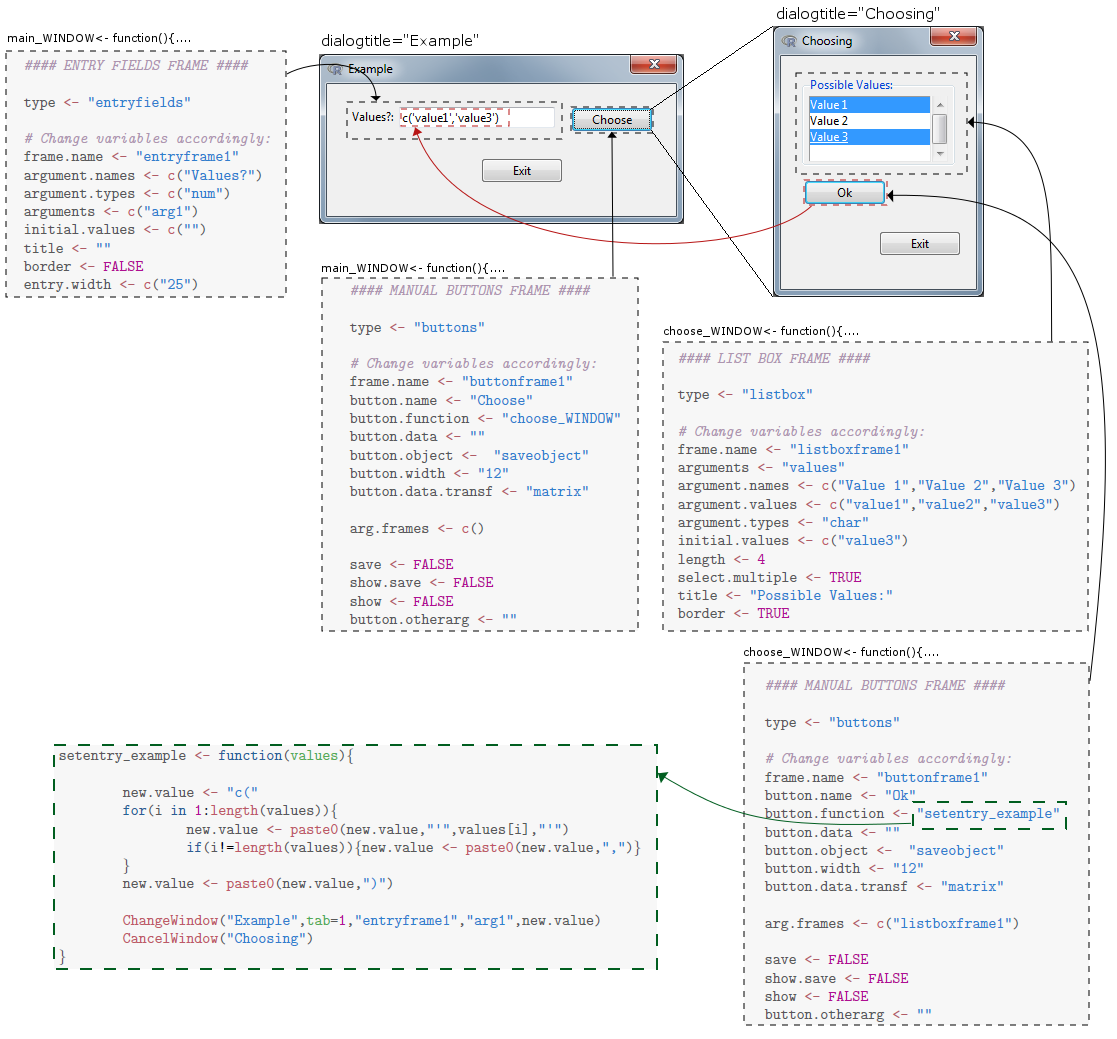
\includegraphics[width=\linewidth]{figures/windowenvir_example.png}
\caption{Window Environments - Example (Code + Window)\label{windowenvir_example}}
\end{figure}


\newpage

\subsection{Extra Functions}
\noindent In this section, you will be able to find some extra functions meant
to be linked to a button or to be used inside functions described in Section
\ref{sec:doitandprint}.
\subsubsection{Save Function}
\texttt{SaveGUI(object.names, init.name="result")}\\ \\
This function will open up a {\it Save} window (Figure \ref{saveGUI}), saving
the chosen \verb|object.names| (vector of the names of the objects to be saved)
in an \verb|.RData| file. The \verb|init.name| variable simply decide the
standard save name which should appear in the save window.
\begin{figure}[H]
\centering
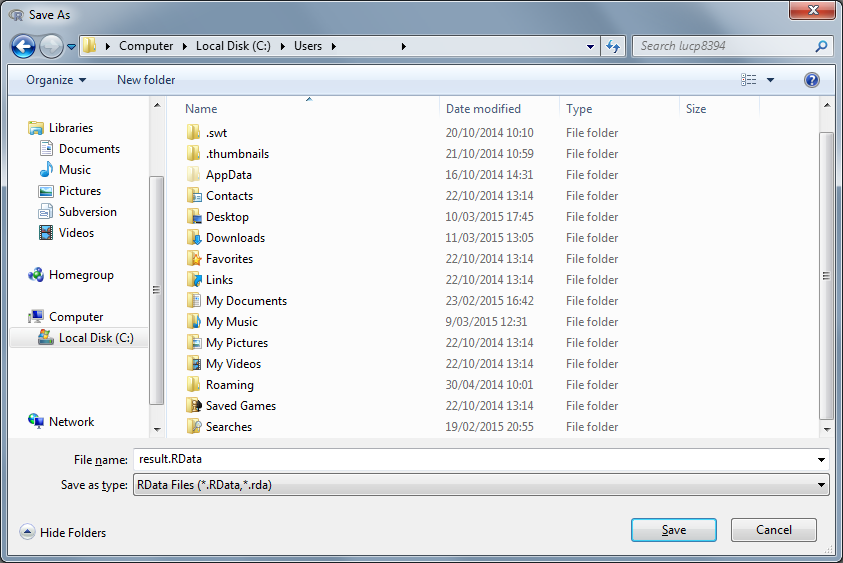
\includegraphics[width=9cm]{figures/saveGUI.png}
\caption{Save Window \label{saveGUI}}
\end{figure}

\subsubsection{Load Function}
\texttt{LoadGUI()}\\ \\
This function opens up a {\it Load} window (Figure \ref{loadGUI}) in which saved
\verb|.RData| objects can be loaded.

\begin{figure}[H]
\centering
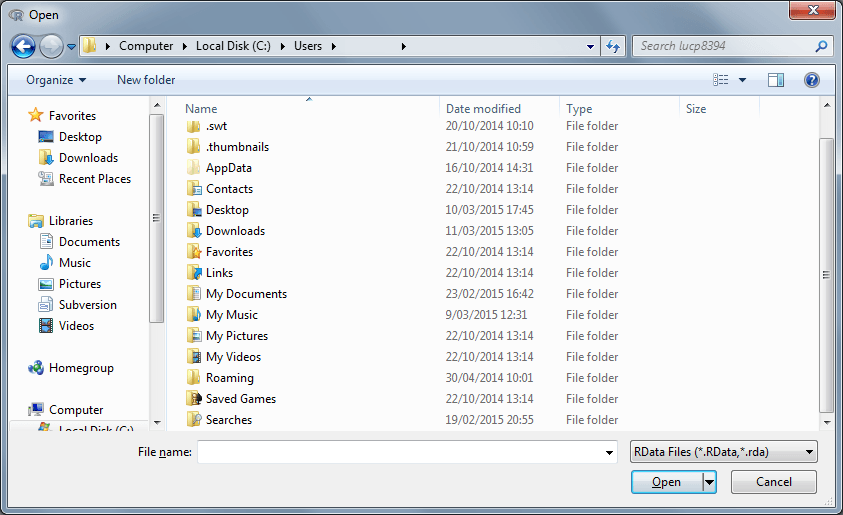
\includegraphics[width=9cm]{figures/loadGUI.png}
\caption{Load Window \label{loadGUI}}
\end{figure}

\newpage
\nocite{*}
\bibliographystyle{asa}
\bibliography{RESTbib}



\newpage
\section{Appendix}
\noindent All the code in the appendix can also be found in R scripts, located
in the \verb|doc| folder of the package.
\subsection{\texttt{.onAttach}-function}
\begin{verbatim}
.onAttach <- function(libname, pkgname){
    if (!interactive()) return()
    putRcmdr("slider.env", new.env())    
    Rcmdr <- options()$Rcmdr
    plugins <- Rcmdr$plugins
    if (!pkgname %in% plugins) {
        Rcmdr$plugins <- c(plugins, pkgname)
        options(Rcmdr=Rcmdr)
        if("package:Rcmdr" %in% search()) {
            if(!getRcmdr("autoRestart")) {
                closeCommander(ask=FALSE, ask.save=TRUE)
                Commander()
            }
        }
        else {
            Commander()
        }
    }
}

\end{verbatim}

\subsection{General Script}
\begin{verbatim}
GUI_WINDOW <- function(list.info=list()){
	
    ##########################
    ## PREAMBLE/INFORMATION ##
    ##########################
	
    dialogtitle <- "This is the title of the window"

    usetabs <- TRUE
    tabnames <- c("Tab 1","Tab 2","Tab 3")
    helppage <- "plot" 
	
    # Do not change these lines
    if(usetabs){ntabs <- length(tabnames)} else {ntabs <- 1}
    new.frames <- .initialize.new.frames(ntabs)
    grid.config <- .initialize.grid.config(ntabs)
    grid.rows <- .initialize.grid.rows(ntabs)
    ###
	
    ##################
    ## GRID BUTTONS ##
    ##################
	
    make.help.button <- TRUE
    make.setwd.button <- TRUE
    make.resetgws.button <- TRUE
    make.seed.button <- TRUE

    ###########
    ## TAB 1 ##
    ###########
    Tab <- 1

    ### 1. ADDING THE FRAMES ###
	
    # Add frames here
	

    ### 2. CONFIGURING THE GRID ###
    grid.config <- .grid.matrix(Tab = Tab, c("frame1","frame2","frame3",NA),
      byrow=TRUE, nrow=2, ncol=2, grid.config=grid.config)


    ### 3. COMBINING THE ROWS ###
    grid.rows <- .combine.rows(Tab = Tab, rows = c(1,2),title = "A nice box: ",
      border = TRUE, grid.rows=grid.rows, grid.config = grid.config)
	
    #############
    ### TAB 2 ###
    #############
    Tab <- 2

    # Repeat what you did for tab 1 for as many tabs as you like...
	
	
    ##################################################################
    ## USE ALL THE ARGUMENTS IN THE GENERAL GUI_TEMPLATE FUNCTION   ##
    ##################################################################
    GUI_template(dialogtitle = dialogtitle, helppage = helppage, make.resetgws.button =
        make.resetgws.button, make.setwd.button = make.setwd.button,
        make.help.button = make.help.button, make.seed.button = make.seed.button,
        usetabs = usetabs, tabnames = tabnames, grid.config = grid.config, grid.rows =
        grid.rows, new.frames = new.frames)
	
}
\end{verbatim}
\subsection{Frame Scripts}
\begin{verbatim}
#### ENTRY FIELDS FRAME ####

type <- "entryfields"

# Change variables accordingly:
frame.name <- "entryframe1"  
argument.names <- c("Argument 1","Argument 2","Argument 3") 
argument.types <- c("num","num","char") 
arguments <- c("arg1","arg2","arg3") 
initial.values <- c(1,2,"a")
title <- "A Title"
border <- FALSE
entry.width <- c("2","2","6")

# Do not change this line:
new.frames <- .add.frame(Tab=Tab,type=type
        ,frame.name=frame.name,argument.names=argument.names
        ,arguments=arguments,initial.values=initial.values
        ,title=title,border=border,entry.width=entry.width
        ,argument.types=argument.types  ,new.frames=new.frames)




#### RADIO BUTTONS FRAME 	####

type <- "radiobuttons"

# Change variables accordingly:
frame.name <- "radioframe1"
argument.names <- c("Button 1","Button 2","Button 3")  
arguments <- c("buttonarg")		
argument.types <- "char" 
argument.values <- c("b1","b2","b3") 
initial.values <- "b3"
title <- "Button Options"
border <- TRUE

# DO NOT CHANGE THIS LINE:
new.frames <- .add.frame(Tab=Tab,type=type
        ,frame.name=frame.name,argument.names=argument.names
        ,arguments=arguments,argument.values=argument.values
        ,initial.values=initial.values,title=title,border=border
        ,new.frames=new.frames,argument.types=argument.types)	


#### CHECK BOXES FRAME  ####

type <- "checkboxes"

# Change variables accordingly:
frame.name <-  "checkboxframe1"
argument.names <- c("Check 1","Check 2","Check 3")  
arguments <- c("checkarg1","checkarg2","checkarg3") 
initial.values <- c(0,1,1)  
title <- "title"
border <- FALSE

# DO NOT CHANGE THIS LINE:
new.frames <- .add.frame(Tab=Tab,type=type
        ,frame.name=frame.name,argument.names=argument.names
        ,arguments=arguments,initial.values=initial.values
        ,title=title,border=border,new.frames=new.frames)


#### VALUE SLIDER FRAME  ####

type <- "valuesliders"

# Change variables accordingly:
frame.name <- "sliderframe1"
argument.names <- c("Slider 1  ","Slider 2  ","Slider 3  ")
arguments <- c("sliderarg1","sliderarg2","sliderarg3") 
initial.values <- c(1,5,10)
from <- c(1,1,1) 
to <- c(5,50,500) 
by <- c(1,10,50)  
length <- c(50,100,150) 
title <- "Title"
border <- TRUE

# DO NOT CHANGE THIS LINE:
new.frames <- .add.frame(Tab=Tab,type=type,
        title=title,border=border,frame.name=frame.name,
        argument.names=argument.names,arguments=arguments,
        initial.values=initial.values,from=from,to=to,by=by,
        length=length,new.frames=new.frames)


#### SPIN BOX FRAME  ####

type <- "spinboxes"

# Change variables accordingly:
frame.name <- "spinboxframe1"
argument.names <- c("Spin Box 1: ","Spin Box 2: ","Spin Box 3: ") 
arguments <- c("spinarg1","spingarg2","spingarg3") 
initial.values <- c(5,10,20)
from <- c(1,5,10)  
to <- c(10,20,30)
by <- c(1,1,1)
entry.width <- "2"  
title <- "Spin Box !"
border <- TRUE

# DO NOT CHANGE THIS LINE:
new.frames <- .add.frame(Tab=Tab,type=type,
        frame.name=frame.name,argument.names=argument.names,
        arguments=arguments,initial.values=initial.values,
        from=from,to=to,by=by,entry.width=entry.width,
        title=title,border=border,new.frames=new.frames)

#### LIST BOX FRAME ####
	
type <- "listbox"
	
# Change variables accordingly:
frame.name <- "listboxframe1"
arguments <- "listboxarg"		 
argument.names <- c("Value 1","Value 2","Value 3")
argument.values <- c("value1","value2","value3")
argument.types <- "char"   		  
initial.values <- c("value3")    
length <- 4 
select.multiple <- FALSE
title <- "A list box:"
border <- TRUE
	
# DO NOT CHANGE THIS LINE:
new.frames <- .add.frame(Tab=Tab,type=type,
    frame.name=frame.name,argument.names=argument.names,
    arguments=arguments,argument.values=argument.values,
    argument.types=argument.types, initial.values=initial.values,
    length=length,select.multiple=select.multiple,
    title=title,border=border,new.frames=new.frames)


#### MANUAL BUTTONS FRAME ####

type <- "buttons"

# Change variables accordingly:
frame.name <- "buttonframe1"  
button.name <- "Button 1"  
button.function <- "buttonfunction" 
button.data <- "d" 
button.object <-  "saveobject" 
button.width <- "12"
button.data.transf <- "matrix" # only matrix available here !

arg.frames <- c("frame1","frame2")

save <- TRUE 
show.save <- TRUE
show <- TRUE
button.otherarg <- ""  # always start with a ,

# Do not change this line: 
new.frames <- .add.frame(Tab=Tab,frame.name=frame.name,
        type=type,button.name=button.name,button.width=button.width,
        button.data.transf=button.data.transf,
        button.function=button.function,button.data=button.data,
        button.object=button.object,button.otherarg=button.otherarg,
        arg.frames=arg.frames,save=save,show=show,show.save=show.save,
        new.frames=new.frames)

\end{verbatim}

\subsection{Example Script}
\begin{verbatim}
plaid_WINDOW <- function(list.info=list()){
	
	##########################
	## PREAMBLE/INFORMATION ##
	##########################
	
	dialogtitle <- "Plaid Biclustering"
	
	
	usetabs <- TRUE
	
	tabnames <- c("Biclustering","Plot & Diagnostics")
	
	if(usetabs){ntabs <- length(tabnames)} else {ntabs <- 1}
	new.frames <- .initialize.new.frames(ntabs)
	grid.config <- .initialize.grid.config(ntabs)
	grid.rows <- .initialize.grid.rows(ntabs)
	
	
	helppage <- "BCPlaid"
	
	
	##################
	## GRID BUTTONS ##
	##################
	
	make.help.button <- TRUE
	make.setwd.button <- FALSE
	make.resetgws.button <- FALSE
	make.seed.button <- TRUE
	
	###########
	## TAB 1 ##
	###########
	Tab <- 1
	
	### 1. ADDING THE FRAMES ###
	
	####		RADIO BUTTONS FRAME 		 ####
	#                               			#
	
	type <- "radiobuttons"
	
	# Change variables accordingly:
	frame.name <- "toclusterframe"
	argument.names <- c("Rows","Columns","Rows & Columns")   
	arguments <- c("cluster")		
	argument.values <- c("r","c","b")
	argument.types <- "char"
	initial.values <- "b" 
	title <- "To Cluster"
	border <- FALSE
	
	# DO NOT CHANGE THIS LINE:
	new.frames <- .add.frame(Tab=Tab,type=type,frame.name=frame.name,
      argument.names=argument.names,arguments=arguments,argument.values=
      argument.values,initial.values=initial.values,title=title,border=border,
      new.frames=new.frames,argument.types=argument.types)	
	
	
	######		  ENTRY FIELDS FRAME 				#####
	#							    		 			#
	
	type <- "entryfields"
	
	# Change variables accordingly:
	frame.name <- "modelframe"  
	argument.names <- c("Model Formula") 
	argument.types <- c("num")
	arguments <- c("fit.model")
	initial.values <- c("y ~ m+a+b")
	title <- "Model"
	border <- FALSE
	entry.width <- c("10")  
	
	# Do not change this line:
	new.frames <- .add.frame(Tab=Tab,type=type,frame.name=frame.name,argument.names=
      argument.names,arguments=arguments,initial.values=initial.values,title=title,
      border=border,entry.width=entry.width,argument.types=argument.types  
      ,new.frames=new.frames)
	
	####		CHECK BOXES FRAME 			  ####
	#                               			 #
	
	type <- "checkboxes"
	
	# Change variables accordingly:
	frame.name <-  "backgroundcheckframe"
	argument.names <- c("Background Layer?") 
	arguments <- c("background") 
	initial.values <- c(1) 
	title <- ""
	border <- FALSE
	
	# DO NOT CHANGE THIS LINE:
	new.frames <- .add.frame(Tab=Tab,type=type,frame.name=frame.name,argument.names=
      argument.names,arguments=arguments,initial.values=initial.values,title=title,
      border=border,new.frames=new.frames)
	
	
	######		  ENTRY FIELDS FRAME 				#####	
	#							    		 			#
	
	type <- "entryfields"
	
	# Change variables accordingly:
	frame.name <- "backgroundentryframe1"  
	argument.names <- c("Shuffle","Back Fit","Max Layes") 
	argument.types <- c("num","num","num")
	arguments <- c("shuffle","back.fit","max.layers")
	initial.values <- c(3,0,20)
	title <- ""
	border <- FALSE
	entry.width <- c("3","3","3")  
	
	# Do not change this line:
	new.frames <- .add.frame(Tab=Tab,type=type,frame.name=frame.name,argument.names=
      argument.names,arguments=arguments,initial.values=initial.values,title=title,
      border=border,entry.width=entry.width,argument.types=argument.types  
      ,new.frames=new.frames)
	
	
	######		  ENTRY FIELDS FRAME 				#####
	#							    		 			#
	
	type <- "entryfields"
	
	# Change variables accordingly:
	frame.name <- "backgroundentryframe2"  
	argument.names <- c("Iteration Startup","Iteration Layer") 
	argument.types <- c("num","num")
	arguments <- c("iter.startup","iter.layer")
	initial.values <- c(5,10)
	title <- ""
	border <- FALSE
	entry.width <- c("3","3")  
	
	# Do not change this line:
	new.frames <- .add.frame(Tab=Tab,type=type,frame.name=frame.name,
      argument.names=argument.names,arguments=arguments,initial.values=
      initial.values,title=title,border=border,entry.width=entry.width,
      argument.types=argument.types  ,new.frames=new.frames)
	
	#### MANUAL BUTTONS FRAME ####

	type <- "buttons"
	
	# Change variables accordingly:
	frame.name <- "plaidbutton"  
	button.name <- "Plaid"  
	button.function <- "biclust" 
	button.data <- "x" 
	button.object <-  "PlaidResult" 
	button.width <- "12"
	button.data.transf <- "matrix" # only matrix available here !
	
	arg.frames <- c("toclusterframe","modelframe","backgroundcheckframe",
      "backgroundentryframe1","backgroundentryframe2")
	
	save <- TRUE 
	show <- TRUE
	show.save <- TRUE
	button.otherarg <- ",method=BCPlaid()" 
	
	# Do not change this line: 
	new.frames <- .add.frame(Tab=Tab,frame.name=frame.name,
			type=type,button.name=button.name,button.width=button.width,
			button.data.transf=button.data.transf,
			button.function=button.function,button.data=button.data,
			button.object=button.object,button.otherarg=button.otherarg,
			arg.frames=arg.frames,save=save,show=show,new.frames=new.frames,
            show.save=show.save)
	
	### 2. CONFIGURING THE GRID ###
	grid.config <- .grid.matrix(Tab=Tab,c("toclusterframe","modelframe",
       "backgroundcheckframe",NA,"backgroundentryframe1","backgroundentryframe2",
       "plaidbutton",NA),byrow=TRUE,nrow=4,ncol=2,grid.config=grid.config)
	
	
	### 3. COMBINING THE ROWS ###
	grid.rows <- .combine.rows(Tab=Tab,rows=c(1),title="Plaid Specifications",
      border=TRUE,grid.rows=grid.rows,grid.config=grid.config)
	grid.rows <- .combine.rows(Tab=Tab,rows=c(2,3),title="Layer Specifications",
      border=TRUE,grid.rows=grid.rows,grid.config=grid.config)
	
	#############
	### TAB 2 ###
	#############
	Tab <- 2
	
	# Repeat what you did for tab 1 for as many tabs as you like...
	
	
	###################################################################
	## USE ALL THE ARGUMENTS IN THE GENERAL GUI_TEMPLATE FUNCTION    ##
	###################################################################
	GUI_template(dialogtitle=dialogtitle,helppage=helppage,make.resetgws.button=
      make.resetgws.button,make.setwd.button=make.setwd.button,make.help.button=
      make.help.button,make.seed.button=make.seed.button,usetabs=usetabs,tabnames=
      tabnames,grid.config=grid.config,grid.rows=grid.rows,new.frames=new.frames)
	
}
\end{verbatim}
\subsection{Window Environment Example}
\begin{verbatim}
main_WINDOW <- function(list.info=list()){
	
	##########################
	## PREAMBLE/INFORMATION ##
	##########################
	
	dialogtitle <- "Example"
		
	usetabs <- FALSE
	
	tabnames <- c("Biclustering","Plot & Diagnostics")
	
	if(usetabs){ntabs <- length(tabnames)} else {ntabs <- 1}
	new.frames <- .initialize.new.frames(ntabs)
	grid.config <- .initialize.grid.config(ntabs)
	grid.rows <- .initialize.grid.rows(ntabs)
		
	helppage <- ""
		
	##################
	## GRID BUTTONS ##
	##################
	
	make.help.button <- FALSE
	make.setwd.button <- FALSE
	make.resetgws.button <- FALSE
	make.seed.button <- FALSE
	
	###########
	## TAB 1 ##
	###########
	Tab <- 1
	
	### 1. ADDING THE FRAMES ###
	
	#### ENTRY FIELDS FRAME ####
	
	type <- "entryfields"
	
	# Change variables accordingly:
	frame.name <- "entryframe1"  
	argument.names <- c("Values?") 
	argument.types <- c("num") 
	arguments <- c("arg1") 
	initial.values <- c("")
	title <- ""
	border <- FALSE
	entry.width <- c("25")
	
	# Do not change this line:
	new.frames <- .add.frame(Tab=Tab,type=type
			,frame.name=frame.name,argument.names=argument.names
			,arguments=arguments,initial.values=initial.values
			,title=title,border=border,entry.width=entry.width
			,argument.types=argument.types  ,new.frames=new.frames)
	

	#### MANUAL BUTTONS FRAME ####
	
	type <- "buttons"
	
	# Change variables accordingly:
	frame.name <- "buttonframe1"  
	button.name <- "Choose"  
	button.function <- "choose_WINDOW" 
	button.data <- "" 
	button.object <-  "saveobject" 
	button.width <- "12"
	button.data.transf <- "matrix" 
	
	arg.frames <- c()
	
	save <- FALSE
	show.save <- FALSE
	show <- FALSE
	button.otherarg <- ""  # always start with a ,
	
	# Do not change this line: 
	new.frames <- .add.frame(Tab=Tab,frame.name=frame.name,
			type=type,button.name=button.name,button.width=button.width,
			button.data.transf=button.data.transf,
			button.function=button.function,button.data=button.data,
			button.object=button.object,button.otherarg=button.otherarg,
			arg.frames=arg.frames,save=save,show=show,show.save=show.save,
			new.frames=new.frames)
	
	### 2. CONFIGURING THE GRID ###
	grid.config <- .grid.matrix(Tab=Tab,c("entryframe1","buttonframe1"),
    byrow=TRUE,nrow=1,ncol=2,grid.config=grid.config)
		
	### 3. COMBINING THE ROWS ###
	
	###################################################################
	## USE ALL THE ARGUMENTS IN THE GENERAL GUI_TEMPLATE FUNCTION    ##
	###################################################################
	GUI_template(dialogtitle=dialogtitle,helppage=helppage,make.resetgws.button=
    make.resetgws.button,make.setwd.button=make.setwd.button,make.help.button=
    make.help.button,make.seed.button=make.seed.button,usetabs=usetabs,tabnames=
    tabnames,grid.config=grid.config,grid.rows=grid.rows,new.frames=new.frames)
	
}

choose_WINDOW <- function(){
	
	##########################
	## PREAMBLE/INFORMATION ##
	##########################
	
	dialogtitle <- "Choosing"
		
	usetabs <- FALSE
	
	tabnames <- c("Biclustering","Plot & Diagnostics")
	
	if(usetabs){ntabs <- length(tabnames)} else {ntabs <- 1}
	new.frames <- .initialize.new.frames(ntabs)
	grid.config <- .initialize.grid.config(ntabs)
	grid.rows <- .initialize.grid.rows(ntabs)
		
	helppage <- ""
	
	##################
	## GRID BUTTONS ##
	##################
	
	make.help.button <- FALSE
	make.setwd.button <- FALSE
	make.resetgws.button <- FALSE
	make.seed.button <- FALSE
	
	###########
	## TAB 1 ##
	###########
	Tab <- 1
	
	### 1. ADDING THE FRAMES ###
		
	#### LIST BOX FRAME ####
	
	type <- "listbox"
	
	# Change variables accordingly:
	frame.name <- "listboxframe1"
	arguments <- "values"		  # should only be 1
	argument.names <- c("Value 1","Value 2","Value 3")
	argument.values <- c("value1","value2","value3")
	argument.types <- "char"   		  # should be only 1
	initial.values <- c("value3")     # Can be 1 or multiple
	length <- 4  #no character , if not given, will take length of names
	select.multiple <- TRUE
	title <- "Possible Values:"
	border <- TRUE
	
	# DO NOT CHANGE THIS LINE:
	new.frames <- .add.frame(Tab=Tab,type=type,
			frame.name=frame.name,argument.names=argument.names,
			arguments=arguments,argument.values=argument.values,
			argument.types=argument.types, initial.values=initial.values,
			length=length,select.multiple=select.multiple,
			title=title,border=border,new.frames=new.frames)
	
	#### MANUAL BUTTONS FRAME ####
	
	type <- "buttons"
	
	# Change variables accordingly:
	frame.name <- "buttonframe1"  
	button.name <- "Ok"  
	button.function <- "setentry_example" 
	button.data <- "" 
	button.object <-  "saveobject" 
	button.width <- "12"
	button.data.transf <- "matrix" 
	
	arg.frames <- c("listboxframe1")
	
	save <- FALSE
	show.save <- FALSE
	show <- FALSE
	button.otherarg <- ""  # always start with a ,
	
	# Do not change this line: 
	new.frames <- .add.frame(Tab=Tab,frame.name=frame.name,
			type=type,button.name=button.name,button.width=button.width,
			button.data.transf=button.data.transf,
			button.function=button.function,button.data=button.data,
			button.object=button.object,button.otherarg=button.otherarg,
			arg.frames=arg.frames,save=save,show=show,show.save=show.save,
			new.frames=new.frames)
	
	
	### 2. CONFIGURING THE GRID ###
	grid.config <- .grid.matrix(Tab=Tab,c("listboxframe1","buttonframe1"),
    byrow=TRUE,nrow=2,ncol=1,grid.config=grid.config)
	
	
	### 3. COMBINING THE ROWS ###
	
	##################################################################
	## USE ALL THE ARGUMENTS IN THE GENERAL GUI_TEMPLATE FUNCTION   ##
	##################################################################
	GUI_template(dialogtitle=dialogtitle,helppage=helppage,make.resetgws.button=
    make.resetgws.button,make.setwd.button=make.setwd.button,make.help.button=
    make.help.button,make.seed.button=make.seed.button,usetabs=usetabs,tabnames=
    tabnames,grid.config=grid.config,grid.rows=grid.rows,new.frames=new.frames)
		
}

setentry_example <- function(values){
	
	new.value <- "c("
	for(i in 1:length(values)){
		new.value <- paste0(new.value,"'",values[i],"'")
		if(i!=length(values)){new.value <- paste0(new.value,",")}
	}
	new.value <- paste0(new.value,")")
	
	ChangeWindow("Example",tab=1,"entryframe1","arg1",new.value)
	CancelWindow("Choosing")
}


\end{verbatim}

\end{document}

%tools::compactPDF("RESTguide.pdf",qpdf="C:/Program Files (x86)/qpdf-5.1.2/bin/qpdf.exe",gs_quality="ebook")
